%!TEX program = xelatex  
%% LyX 2.2.0rc1 created this file.  For more info, see http://www.lyx.org/.
%% Do not edit unless you really know what you are doing.
% test the gitlab function
% test gitlab push function
\documentclass[english,justified]{tufte-book}
\usepackage[T1]{fontenc}
\usepackage{geometry}
\geometry{verbose}
\setcounter{secnumdepth}{1}
\usepackage{textcomp}
\usepackage{amsmath}
\usepackage{amssymb}
\usepackage{babel}
\usepackage{xcolor}

%%%%%%%%%%%%%%%%%%%%%%%%%%%%%%%%  including the \maketitle %%%%%%%%%%%%%%%%%%
\usepackage{ifxetex}
\ifxetex
  \newcommand{\textls}[2][5]{%
    \begingroup\addfontfeatures{LetterSpace=#1}#2\endgroup
  }
  \renewcommand{\allcapsspacing}[1]{\textls[15]{#1}}
  \renewcommand{\smallcapsspacing}[1]{\textls[10]{#1}}
  \renewcommand{\allcaps}[1]{\textls[15]{\MakeTextUppercase{#1}}}
  \renewcommand{\smallcaps}[1]{\smallcapsspacing{\scshape\MakeTextLowercase{#1}}}
  \renewcommand{\textsc}[1]{\smallcapsspacing{\textsmallcaps{#1}}}
  \usepackage{fontspec}
\fi

%%%%%%%%%%%%%%%% uncomment this line if you prefer colored hyperlinks 
%%%%%%%%%%%%%%%% (e.g., for onscreen viewing)
\usepackage{hyperref}
\hypersetup{colorlinks}

%%%%%%%%%%%%%%%%%%%% For graphics / images
\usepackage{graphicx}
\setkeys{Gin}{width=\linewidth,totalheight=\textheight,keepaspectratio}
\graphicspath{{graphics/}}

% The fancyvrb package lets us customize the formatting of verbatim
% environments.  We use a slightly smaller font.
\usepackage{fancyvrb}
\fvset{fontsize=\normalsize}

% chinese words package
%\usepackage{fontspec, xunicode, xltxtra}  
%\setmainfont{Hiragino Sans GB} 

\usepackage{xeCJK}
\setCJKmainfont{STSong}     

% Generates the index
\usepackage{makeidx}
\makeindex

%%%%%%%%%%%%%%%  title information
\title{Note Book}
\author[]{Fu Li}
\publisher{Publisher of This Book}

\usepackage{shorttoc}

\renewcommand*\contentsname{Contents (detailed)}


\begin{document}
\maketitle

%% short contents
\pdfbookmark[1]{Contents}{toc}
\shorttoc{Contents}{0}
\cleardoublepage

%% detailed contents with depth of 2
\pdfbookmark[1]{Contents (detailed)}{toc (detailed)}
\setcounter{tocdepth}{1}
\tableofcontents


\chapter{CO2}

\begin{itemize}

\item many papers talk about the line intensity measurements around 1.6 μm

\end{itemize}



The vibrational term values $G(v)$,[note 3] for an anharmonic oscillator are given, to a first approximation, by

\[{\displaystyle G(v)=\omega _{e}\left(v+{1 \over 2}\right)-\omega _{e}\chi _{e}\left(v+{1 \over 2}\right)^{2}\,}\]
where v is a vibrational quantum number, ωe is the harmonic wavenumber and χe is an anharmonicity constant.

When the molecule is in the gas phase, it can rotate about an axis, perpendicular to the molecular axis, passing through the centre of mass of the molecule. The rotational energy is also quantized, with term values to a first approximation given by
\[F_{v}(J)=B_{v}J\left(J+1\right)-DJ^{2}\left(J+1\right)^{2}\]

where J is a rotational quantum number and D is a centrifugal distortion constant. The rotational constant, Bv depends on the moment of inertia of the molecule, Iv, which varies with the vibrational quantum number, v
\[B_{v}={h \over {8\pi ^{2}cI_{v}}};\quad I_{v}={\frac  {m_{A}m_{B}}{m_{A}+m_{B}}}d_{v}^{2}\]

where mA and mB are the masses of the atoms A and B, and d represents the distance between the atoms. The term values of the ro-vibrational states are found (in the Born–Oppenheimer approximation) by combining the expressions for vibration and rotation.

\[{\displaystyle G(v)+F_{v}(J)=\left[\omega _{e}\left(v+{1 \over 2}\right)+B_{v}J(J+1)\right]-\left[\omega _{e}\chi _{e}\left(v+{1 \over 2}\right)^{2}+DJ^{2}(J+1)^{2}\right]}\]

The first two terms in this expression correspond to a harmonic oscillator and a rigid rotor, the second pair of terms make a correction for anharmonicity and centrifugal distortion. A more general expression was given by Dunham.

The selection rule for electric dipole allowed ro-vibrational transitions, in the case of a diamagnetic diatomic molecule is etc.
$ \Delta v=\pm 1\ (\pm 2,\pm 3,{\textit {etc.}},\Delta J=\pm 1$
The transition with Δv=±1 is known as the fundamental transition. The selection rule has two consequences.

\begin{itemize}
\item Both the vibrational and rotational quantum numbers must change. The transition : $\Delta v=\pm 1,\Delta J=0$ (Q-branch) is forbidden

\item The energy change of rotation can be either subtracted from or added to the energy change of vibration, giving the P- and R- branches of the spectrum, respectively.
\end{itemize}


\subsection{For $CO_{2}$}
\begin{enumerate}
\item transition $\left(0001\right)-\left(10001\right),960.9cm^{-1},4.26\mu m,70.42Thz,\left\langle \wp_{ab}\right\rangle ^{2}=15*10^{-4}D^{2},$
\item transition $\left(0001\right)-\left(10002\right),1063.7cm^{-1},9.4\mu m,31.89Thz,\left\langle \wp_{ab}\right\rangle ^{2}=12*10^{-4}D^{2},$
\item transition $\left(0001\right)-\left(0000\right),2349.1cm^{-1},9.4\mu m,31.89Thz,\left\langle \wp_{ab}\right\rangle ^{2}=0.103D^{2},$
\end{enumerate}
Transition between $\left(0001\right)-\left(10001\right),\left\langle \wp_{ab}\right\rangle ^{2}=15*10^{-4}D^{2}$
to relized 10Mhz

\begin{align*}
I & =\frac{5.4}{15}*10^{4}W/cm^{2}\\
 & =3.6*10^{3}W/cm^{2}
\end{align*}

note: for Rubidium 87

D2$\left(5^{2}S_{1/2}\rightarrow5^{2}P_{3/2}\right)$Transition Dipole
Matrix Element 

$4.22752(87)ea_{0}=3.58424(74)\times10^{-29}C\cdot m=10.8D$

To relized 10Mhz, need $5.4\frac{W}{cm^{2}}$

\subsection{WAVENUMBER/WAVELENGTH CONVERTER}

\begin{align*}
xnm & =10,000,000/xcm^{-1}\\
ycm^{-1} & =10,000,000/ynm
\end{align*}


\chapter{Computer Languge}
\label{ch:Computer Languge}

\section{blender}

Open the blender in the terminal as 
\begin{verbatim}
/Applications/blender/blender.app/Contents/MacOS/blender
\end{verbatim}
So the system console works.

\begin{itemize}
\item everytime you move the object, there is a python code appares at the top of the scene, which could be copy into the Scripting.
\item  next
\end{itemize}


\section{OSX}

Find the file location:
\begin{verbatim}
Method 1: From the Terminal, type "open -a Finder /usr/local/bin".

Method 2: From Finder's "Go" menu, select "Go to folder...". That'll bring up a window in which you can type "/usr/local/bin".
\end{verbatim}

\subsection{burn orignal.iso into usb}

in the terminal input those following command:

\begin{itemize}
\item diskutil list
\item diskutil unmountDisk /dev/disk2\footnote{The usb disk}   
\item sudo dd if=orignal.iso\footnote{you can drag the file into here} of=/dev/disk2\footnote{The usb disk} bs=1m
\end{itemize}

Note:
the procession will take 20-30 mins.

\section{python}

Using pypy 
\begin{verbatim}
At the command line, instead of:
python my_program.py

Use:
path/to/where/you/installed/pypy my_program.py
\end{verbatim}

\section{Fortran}

The intriduction

Firstly, you need to know how to run the Fortran independtly, not with communication with python or others. Such as: gfortran name.f90 -llapack -lblas.

The subroutine programe of Fortran could be used to improve the calculation speed of python. There are two ways to do this job.

\begin{itemize}
	\item f2py, which is general way to compile fortran to .os file that could be called in python \url{https://docs.scipy.org/doc/numpy-dev/f2py/}.
	\item jupyter, the previser version is ipyhotn, which give a more easy and simple way to call fortran subroutine in python when subroutine programe is short and without using libs \url{http://nbviewer.jupyter.org/github/mgaitan/fortran_magic/blob/master/documentation.ipynb}.
\end{itemize}

Note: Jupyter is very good and useful tool to develope the programe, because that it could show the calculation result within the code. Moreover, you also could edit the word in bolcks, which is similar with Mathematica files. But, sometimes, I suspect its calculaton result. I feel that I cannot control the memory space. I have tested the case that fortran subroutin contains the lib. Even I delete the lib, it still give the right result. But if I just change to the wrong subroutine name, it does not work. So, I think it does not totally clear the previous memory when you run it second time.  


There are many good subroutine programes we could use, please see the web : \url{https://people.sc.fsu.edu/~jburkardt/index.html}


Run the excutable file
\begin{verbatim}
./a.out
\end{verbatim}


\subsection{Package }

Today, I’ve installed two popular packages \footnote{ \url{http://fortranwiki.org/fortran/show/Libraries}}:

LAPACK, see http://www.netlib.org/lapack/

BLAS, see http://www.netlib.org/blas/

Both packages are required when you deal with linear algebra operations, e.g. solving linear equation systems. Originally, both packages were written in FORTRAN, but I want to use them coding in C++. The solution is to create a libraray! There’re a few steps to consider while installing the packages. First, you have to install BLAS, because LAPACK requires it. If you have downloaded both packages, unzip them. Switch to the BLAS folder and execute
\begin{verbatim}
\$ make
\end{verbatim}
to compile all fortran files. After that, execute

\begin{verbatim}
 \$ mv blas_LINUX.a libblas.a
\end{verbatim}
to rename the created library. Now, you created a library called “libblas.a”. You just copy that file to your library folder. Therefore execute the following command

\begin{verbatim}
 sudo cp libblas.a /usr/local/lib/
\end{verbatim}
Et voila. You’ve installed the BLAS package. 

Now switch to the LAPACK folder and adjust the file “make.inc”. If you set all parameter correctly, execute the command

\begin{verbatim}
sudo cp make.inc.example make.inc
sudo make blaslib
sudo make
\end{verbatim}

\textbf{sudo make blaslib} produces the \textbf{librefblas.a} file, then change the name, and copy it to the /usr/local/lib/.\footnote{All libs shoud be added into \textbf{/usr/local/lib/}, where is the defort location for gfortran libs. In this way, the compile is very esay; \textbf{gfortran name.f90 -llapack -lblas}}

\begin{verbatim}
 sudo cp librefblas.a libblas.a
 sudo cp libblas.a /usr/local/lib/
 sudo cp liblapack.a /usr/local/lib/
\end{verbatim}

In this way, we have put two libs "liblapack.a and libblas.a" into the PATH. Congratulation, you’ve installed BLAS and LAPACK on Mac OS!

Compile the .f90 file:

\textbf{gfortran name.f90 -llapack -lblas}


中文参考 \url{http://www.poluoluo.com/server/200807/19872.html}: 如果编译和测试顺利的话会在源代码的根目录下生成三个文件 liblapack.a、libblas.a、libtmglib.a. liblapack.a 和 libblas.a 就是我们所需要的库函数。它们的使用有两种途径:

a)拷贝liblapack.a 和 libblas.a 到 /usr/local/lib/ 目录下,或者它们所在的目录加入到 /usr/local/lib/环境变量中,或者在编译时候加上 “-L lapack所在目录/” 选项。编译的时候加上编译选项 -llapack -lblas.
 
b) 编译的时候直接把 liblapack.a 和 libblas.a 一起同需要编译的代码一起编译。比如 要编译的文件为 main.f90 编译器为 gfortran.  \textbf{gfortran main.f90 lapack.a blas.a}

GFORTRAN guesses the source code formatting based on the file extension. For .f90 files, it will assume it’s working with FORTRAN 90 source code and use free formatting rules. For .f and .for files, it will assume the file is F77 source code and use fixed formatting rules. I believe this is the problem you’re experiencing. You can override the defaults with -ffixed-form and -ffree-form.

Using \textit{xcode},

\begin{itemize}
\item  choosing "Type" to be "Fortran 90 Source" could make the code color, but not  "Fortran 77 Source" and "Fortran Source"
\item  only one file could exist
\item  only could comple the ".f90" file 

\end{itemize}

\subsection{Modern Fortran Explained}

the Fortran 90 standard was much more a development of the language, introducing features which were new to Fortran, but were based on experience in other languages. The main features of Fortran 90 were, first and foremost, the array language and abstract data types. Last but not least were the new free source form, an improved style of attribute-oriented specifications, the implicit none statement, and a mechanism for identifying redundant features for subsequent removal from he language.

One list contains the deleted features, those that have been removed. Since Fortran 90 contained the whole of Fortran 77, this list was empty for Fortran 90 but was not for Fortran 95. The obsolescent features that were deleted from Fortran 95 are still being supported by most compilers, because of the demand for old tried and tested programs to continue to work. Thus, the concept of obsolescence is really not working as intended, but at least it gives a clear signal that certain features are outmoded, and should be avoided in new programs and not be taught to new programmers.

A drawback of the Fortran 77 standard was that it made no statement about requiring processors to provide a means to detect any departure from the allowed syntax by a program, as long as that departure did not conflict with the syntax rules defined by the standard. The new standards are written in a different style from the old one. The syntax rules are expressed in a form of BNF with associated constraints, and the semantics are described by the text.

Any Fortran statement (that is not part of a compound statement) may be labelled, in order to be able to identify it. For some statements a label is mandatory. A statement label precedes the statement, and is regarded as a token. The label consists of from one to five digits, one of which must be nonzero. An example of a labelled statement is

100 continue

Leading zeros are not significant in distinguishing between labels. For example, 10 and 010 are equivalent.

\begin{verbatim}
selected_int_kind(6) 
\end{verbatim}
is an intrinsic inquiry function call, and it returns a kind parameter value that yields the range \textbf{−999999 to 999999} with the least margin

The default kind consists of a string of characters enclosed in a pair of either apostrophes or quotation marks. 

If expr is not of the same type or kind as variable, it will be converted to that type and kind before the assignment is carried out.

$i <0$ integer relational expression

In this case, and whenever either or both of the two components consist of numeric expressions, the rules state that the components are to be evaluated separately, and converted to the type and kind of their sum before the comparison is made.

\begin{verbatim}
character(len=5) :: fill
 fill(1:4) = ’AB’
\end{verbatim}
$fill(1:4)$ will have the value ABbb (where b stands for a blank character). The value of $fill(5:5)$ remains undefined, that is, it contains no specific value and should not be used in an expression. As a consequence, fill is also undefined.

The most important form is that of a block construct, that is a construct which begins with an initial keyword statement, may have intermediate keyword statements, and ends with a matching terminal statement, and that may be entered only at the initial statement. 

\begin{verbatim}
[name:] do
\end{verbatim}
In practice, a means to exit from an endless loop is required, and this is provided in the form of the exit statement:

\begin{verbatim}
exit [name]
\end{verbatim}

where name is optional and is used to specify from which do construct the exit should be taken in the case of nested constructs.

\begin{verbatim}
cycle [name]
\end{verbatim}

which transfers control to the end do statement of the corresponding construct.

A complete program must, as a minimum, include one \textbf{main program}. This may contain statements of the kinds that we have met so far in examples, but normally its most important statements are invocations or calls to subsidiary programs known as subprograms. A subprogram defines a \textbf{function} or a \textbf{subroutine}. 

Another way to stop program execution is to execute a \textbf{stop} statement. This statement may appear in the main program or any subprogram. A well-designed program normally returns control to the main program for program termination, so the \textbf{stop} statement should appear there. However, in applications where several \textbf{stop} statements appear in various places in a complete program, it is possible to distinguish which of the \textbf{stop} statements has caused the termination by adding to each one a stop code consisting of a default character constant or a string of up to five digits whose leading zeros are not significant.
\begin{verbatim}
   stop
   stop ’Incomplete data. Program terminated.’
   stop 12345
\end{verbatim}

\section{linux}

pwd, print working directory, which outputs (displays) the current directory.\\
cd,  change your current direc- tory (see above) will change the prompt but will not display any output. \\
mkdir, Make a new directory\\
touch, Make a new empty file\\
cp, Copy a file\\
mv, Move a file\\
rm, Remove a file or directory (learn about the -r option)\\
less, Show the contents of a file in a scrolling buffer\\
\vspace{5mm}
Fortunately, most commands have a manual. To read, use the man command. Pass the name of the command you want to learn about as it’s only argument. For instance to learn more about ls, run\\
man ls


\section{C++}

As with all formatting manipulators, you must include the header file iomanip to use setprecision. 

- You can control the number of significant digits with which floating-point values are displayed by using the setprecision manipulator. 
The number inside the parentheses after the word setw specifies the field width for the value immediately following it. 
\begin{verbatim}
* cout << setprecision(2) << fixed; 
\end{verbatim}

- When the fixed manipulator is used, all floating point numbers that are subsequently printed will be displayed in fixed point notation, with the number of digits to the right of the decimal point specified by the setprecision manipulator. 

- When the fixed and setprecision manipulators are used together, the value speci- fied by the setprecision manipulator will be the number of digits to appear after the decimal point, not the number of significant digits. 

\begin{verbatim}
* // Display the sales figures. 
* 23  cout << "\nSales Figures\n"; 
* 24  cout << "-------------\n"; 
* 25  cout << setprecision(2) << fixed; 
* 26  cout << "Day 1: " << setw(8) << day1 << endl; 
* 27  cout << "Day 2: " << setw(8) << day2 << endl; 
* 28  cout << "Day 3: " << setw(8) << day3 << endl; 
* 29  cout << "Total: " << setw(8) << total << endl; 
* 30  return 0; 

\end{verbatim}

Pointers 


- 9.1 Getting the Address of a Variable

Getting the address of a variable is accomplished with an operator in C++. When the address operator ($\&$) is placed in front of a variable name, it returns the address of that variable. Here is an expression that returns the address of the variable amount: 

\begin{verbatim}
* & amount 
And here is a statement that displays the variable’s address on the screen: 
* cout << & amount; 
\end{verbatim}



\chapter{Latex}

\section{ MacTeX 配置中文支持}

目前来说,结合 xeCJK 宏包使用 XeLaTeX 编译,应该是最方便的方式了。 XeLaTeX 要求 .tex 文档保存为 UTF-8 编码。所以要做的事情只有两件 \footnote{http://liam0205.me/2014/11/02/latex-mactex-chinese-support/}:

\begin{enumerate}
	\item 配置一个 UTF-8 的编辑环境;
    \item 用 xeCJK 的语法选择合适的字体。
\end{enumerate}

XeTeX 在 Mac OS X 下的行为和 Windows/Linux 下不大一样。Mac 底下,XeTeX 并不使用 fontconfig 库来搜索字体,所以我们没法在终端里通过 fc-list 命令来查看可用的字体列表。不过 Mac 里提供了名为「字体册」的程序,来列出系统中所有可用的字体信息。

其实这样的设计挺讨厌的,TeX Live 自带了许多开源字体,因此没有办法很好地使用。必须用字体名而不是字族名来调用这些字体,实在是不太方便。当然,如果有需要,我们可以把 TeX 里自带的这些开源字体用硬链接的方式,添加到 Mac 的字体目录下。

打开字体册程序,找到需要的字体信息:

\begin{figure*}
	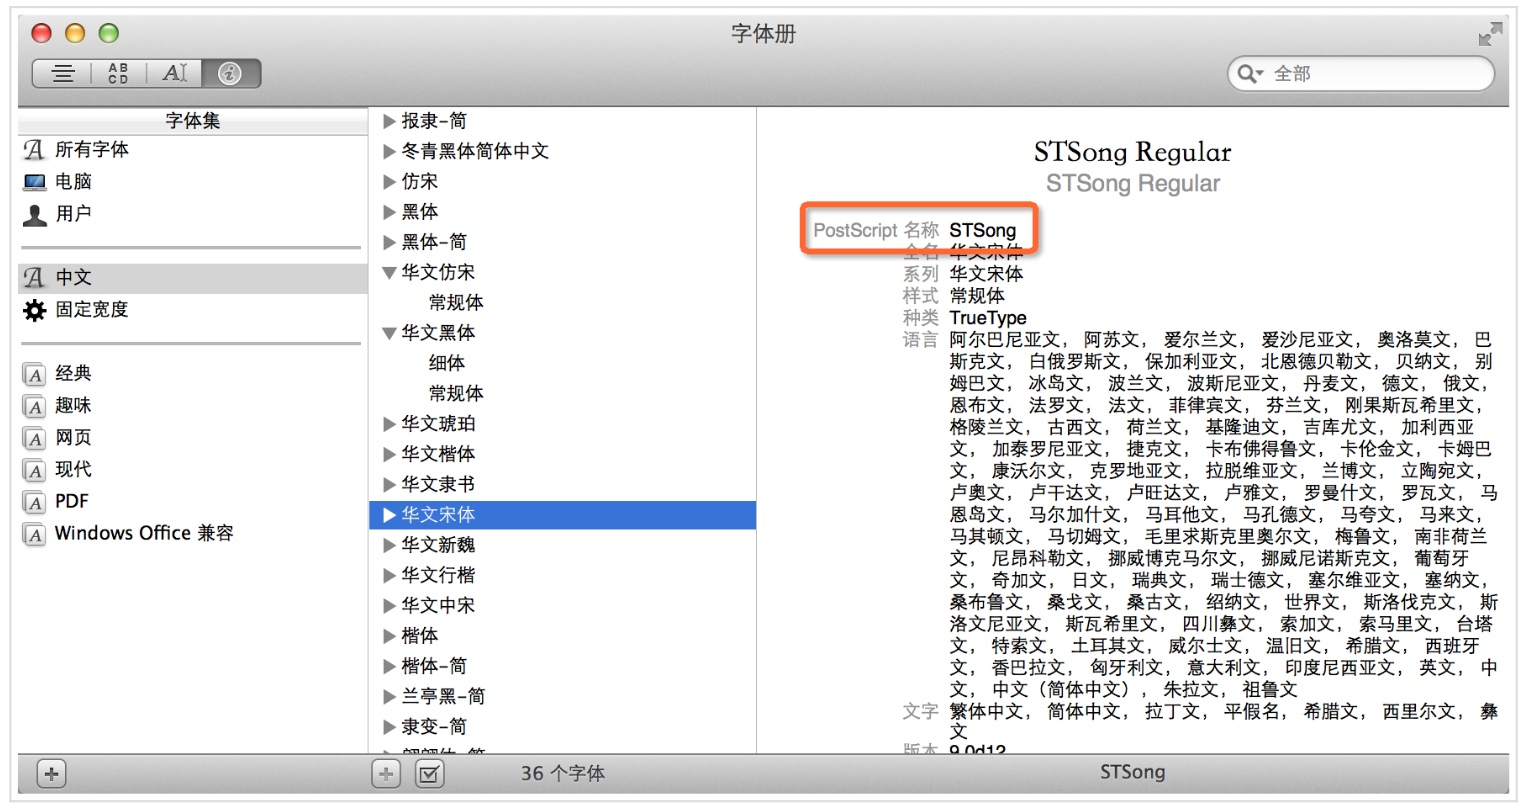
\includegraphics{chapter/CL_fig/mac字体}
	\caption{mac字体}
\end{figure*}

这里的 PostScript 名称就是我们需要的信息,我们记下华文宋体的名字:「\colorbox{red}{STSong}」。你还可以按需找到其他字体的名字,比如华文中宋、华文楷体、华文黑体等字体的名字。

Note: \colorbox{red}{在mac里面不是SimSun字体,而是STSong}, 在win下面是STSong。


\section{texmaker}

\subsection{short cut}

see the \textbf{texmaker $\rightarrow$ preference $\rightarrow$ Shortcut}

\section{compile latex using terminal}

latexmk -xelatex filename\footnote{1. you should cd to the filename dic. 2.the compile speed is faster, I think, using this way.}

You need to compile the file two times to generate the table of content/figures/tables lists. 

\section{Latex + sublime}

package "Latexing" is for color display.

\begin{verbatim} 
%!TEX program = xelatex  
\end{verbatim} \sidenote{determine the engine: xelatex}


\begin{verbatim}
\usepackage{fontspec, xunicode, xltxtra}  
\setmainfont{Hiragino Sans GB}  

or using 

\usepackage{xeCJK}
\setCJKmainfont{SimSun}

\end{verbatim} \sidenote{chinese words}

\begin{verbatim}
\usepackage{xcolor}
\usepackage{hyperref}
  \hypersetup{pagebackref,
              backref,
              colorlinks,
              linkcolor=blue,
              anchorcolor=red,
              citecolor=blue,
              urlcolor=magenta} 
\end{verbatim} \sidenote{hyperlink setup}
                 
\begin{verbatim}                 
\usepackage{geometry}
\newgeometry{left=1in,
             right=1in,
             top=1in,
             bottom=1in,
             headsep=1cm,
             marginparwidth=85pt,
             marginparsep=11pt}             
\end{verbatim} \sidenote{Page Layout}

\begin{figure*}
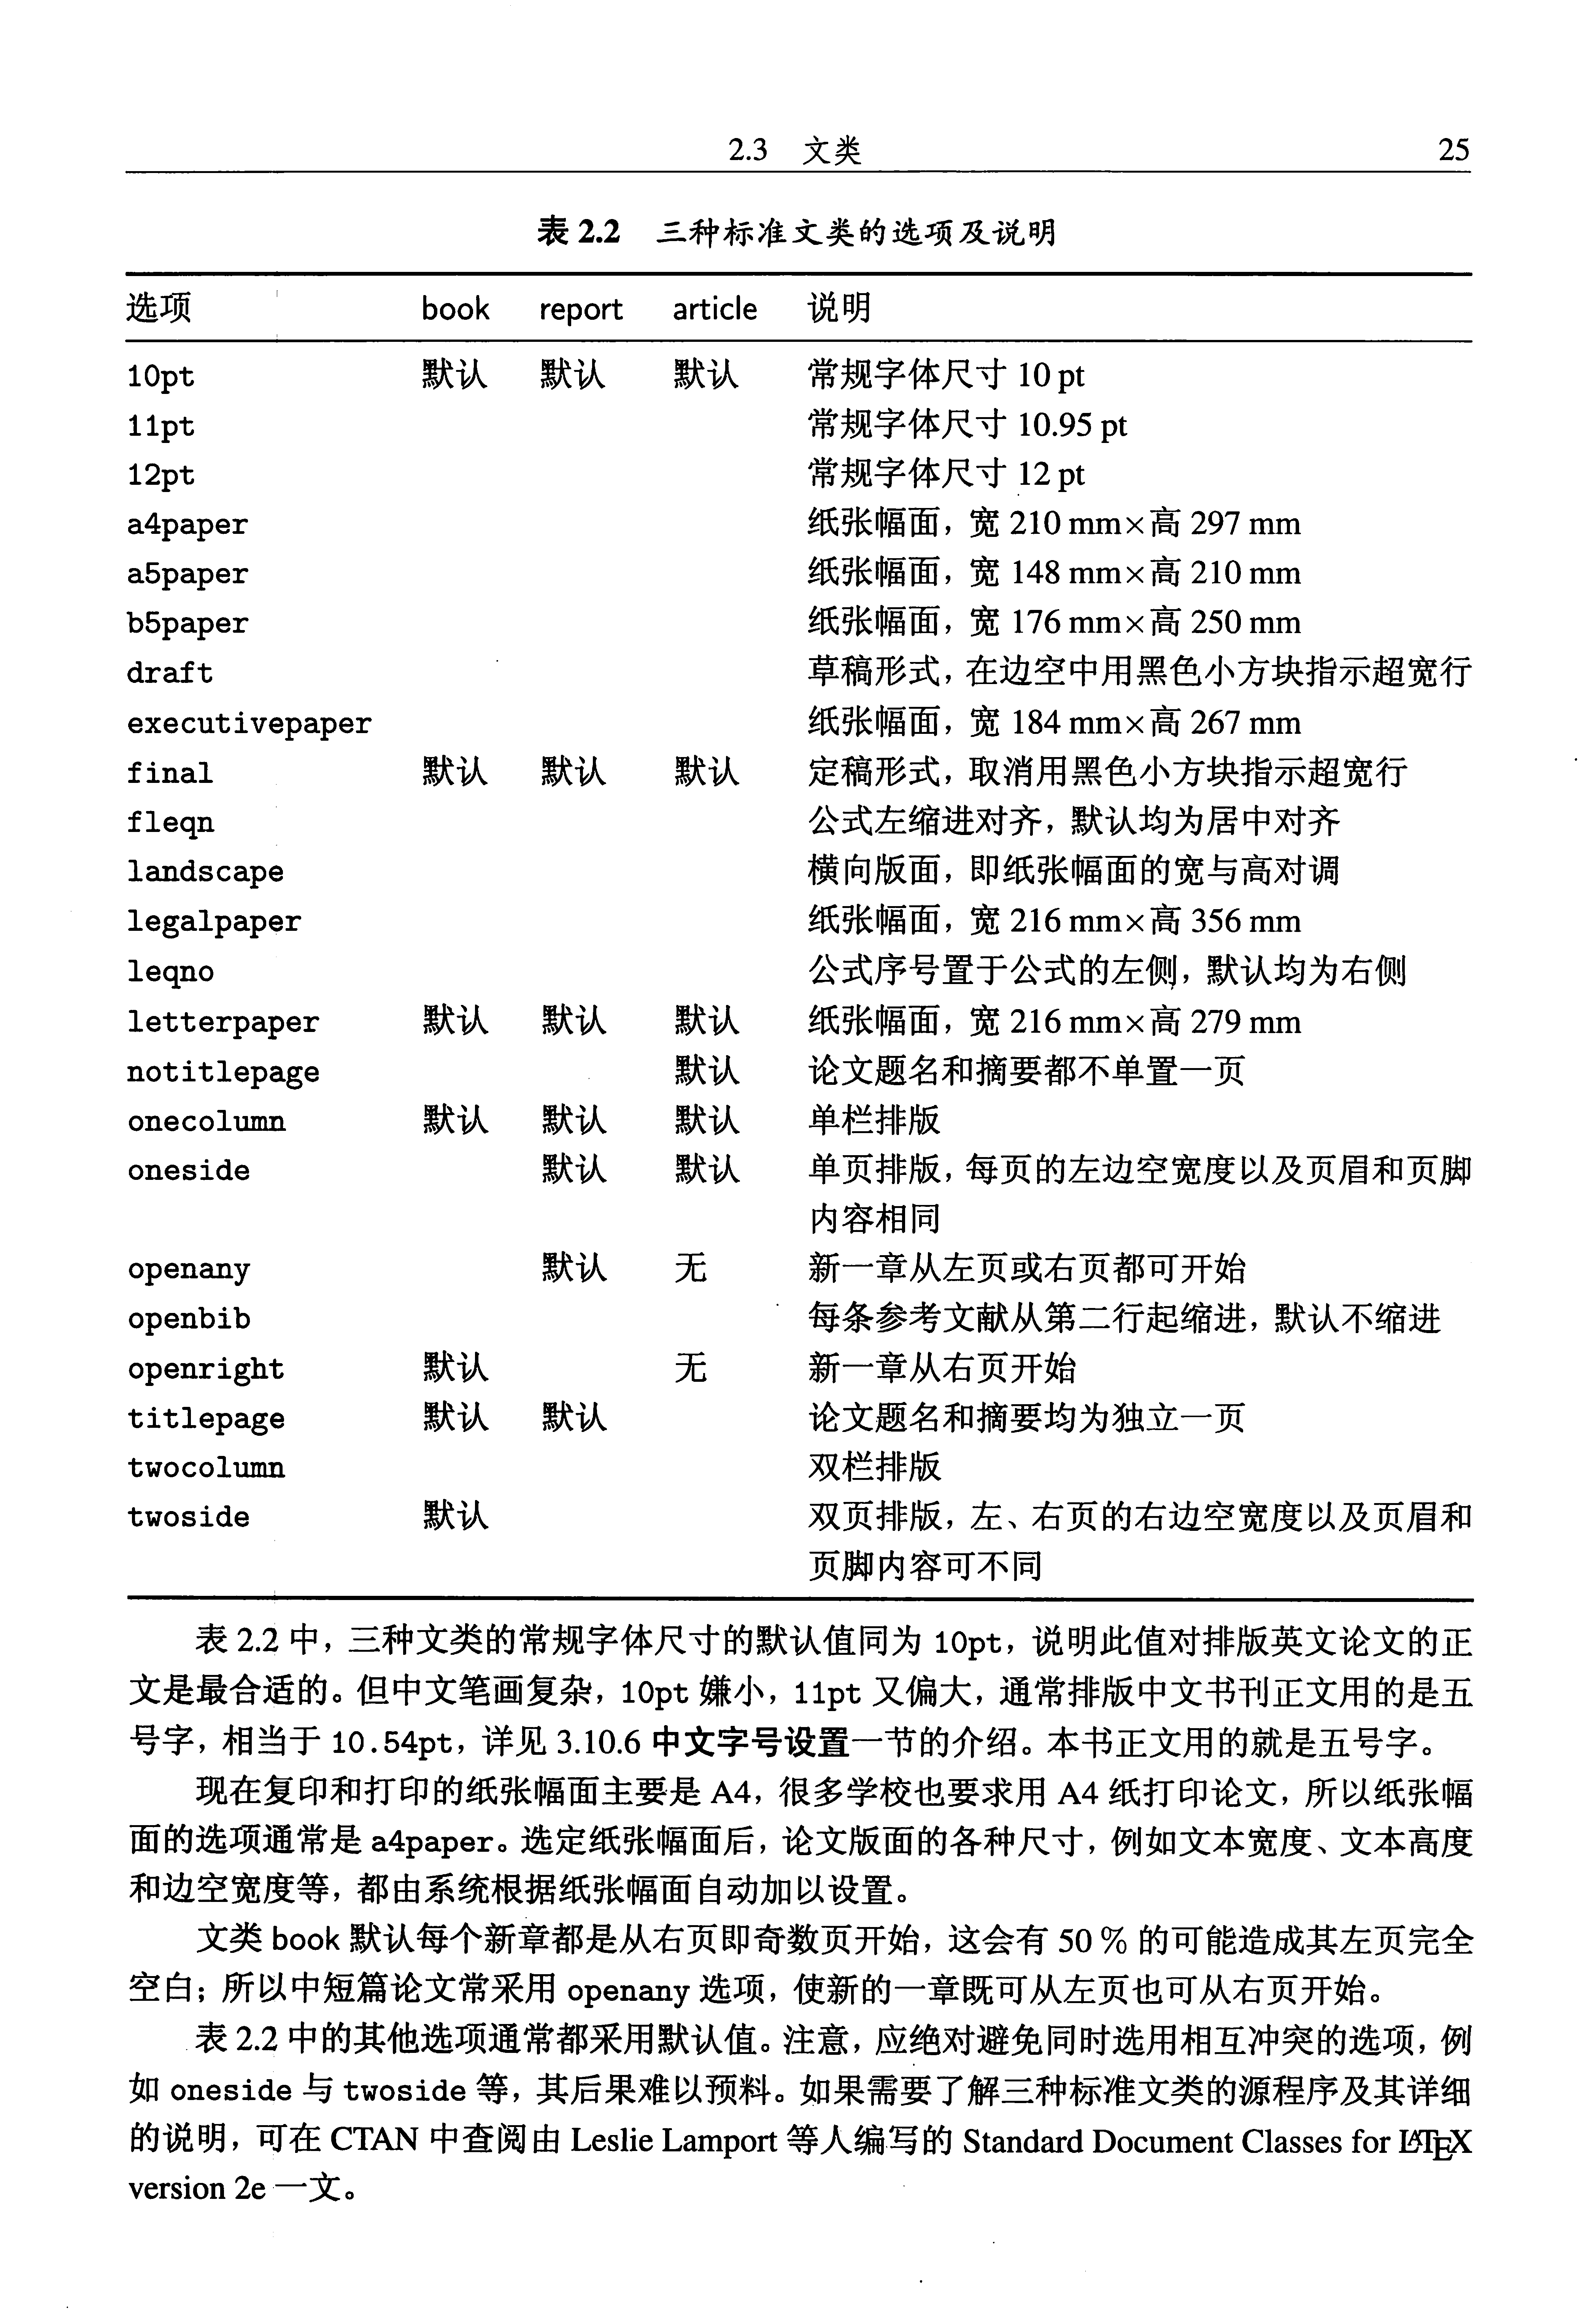
\includegraphics{figures/文类.jpg}
      \caption{文类}
\end{figure*}

\begin{figure*}
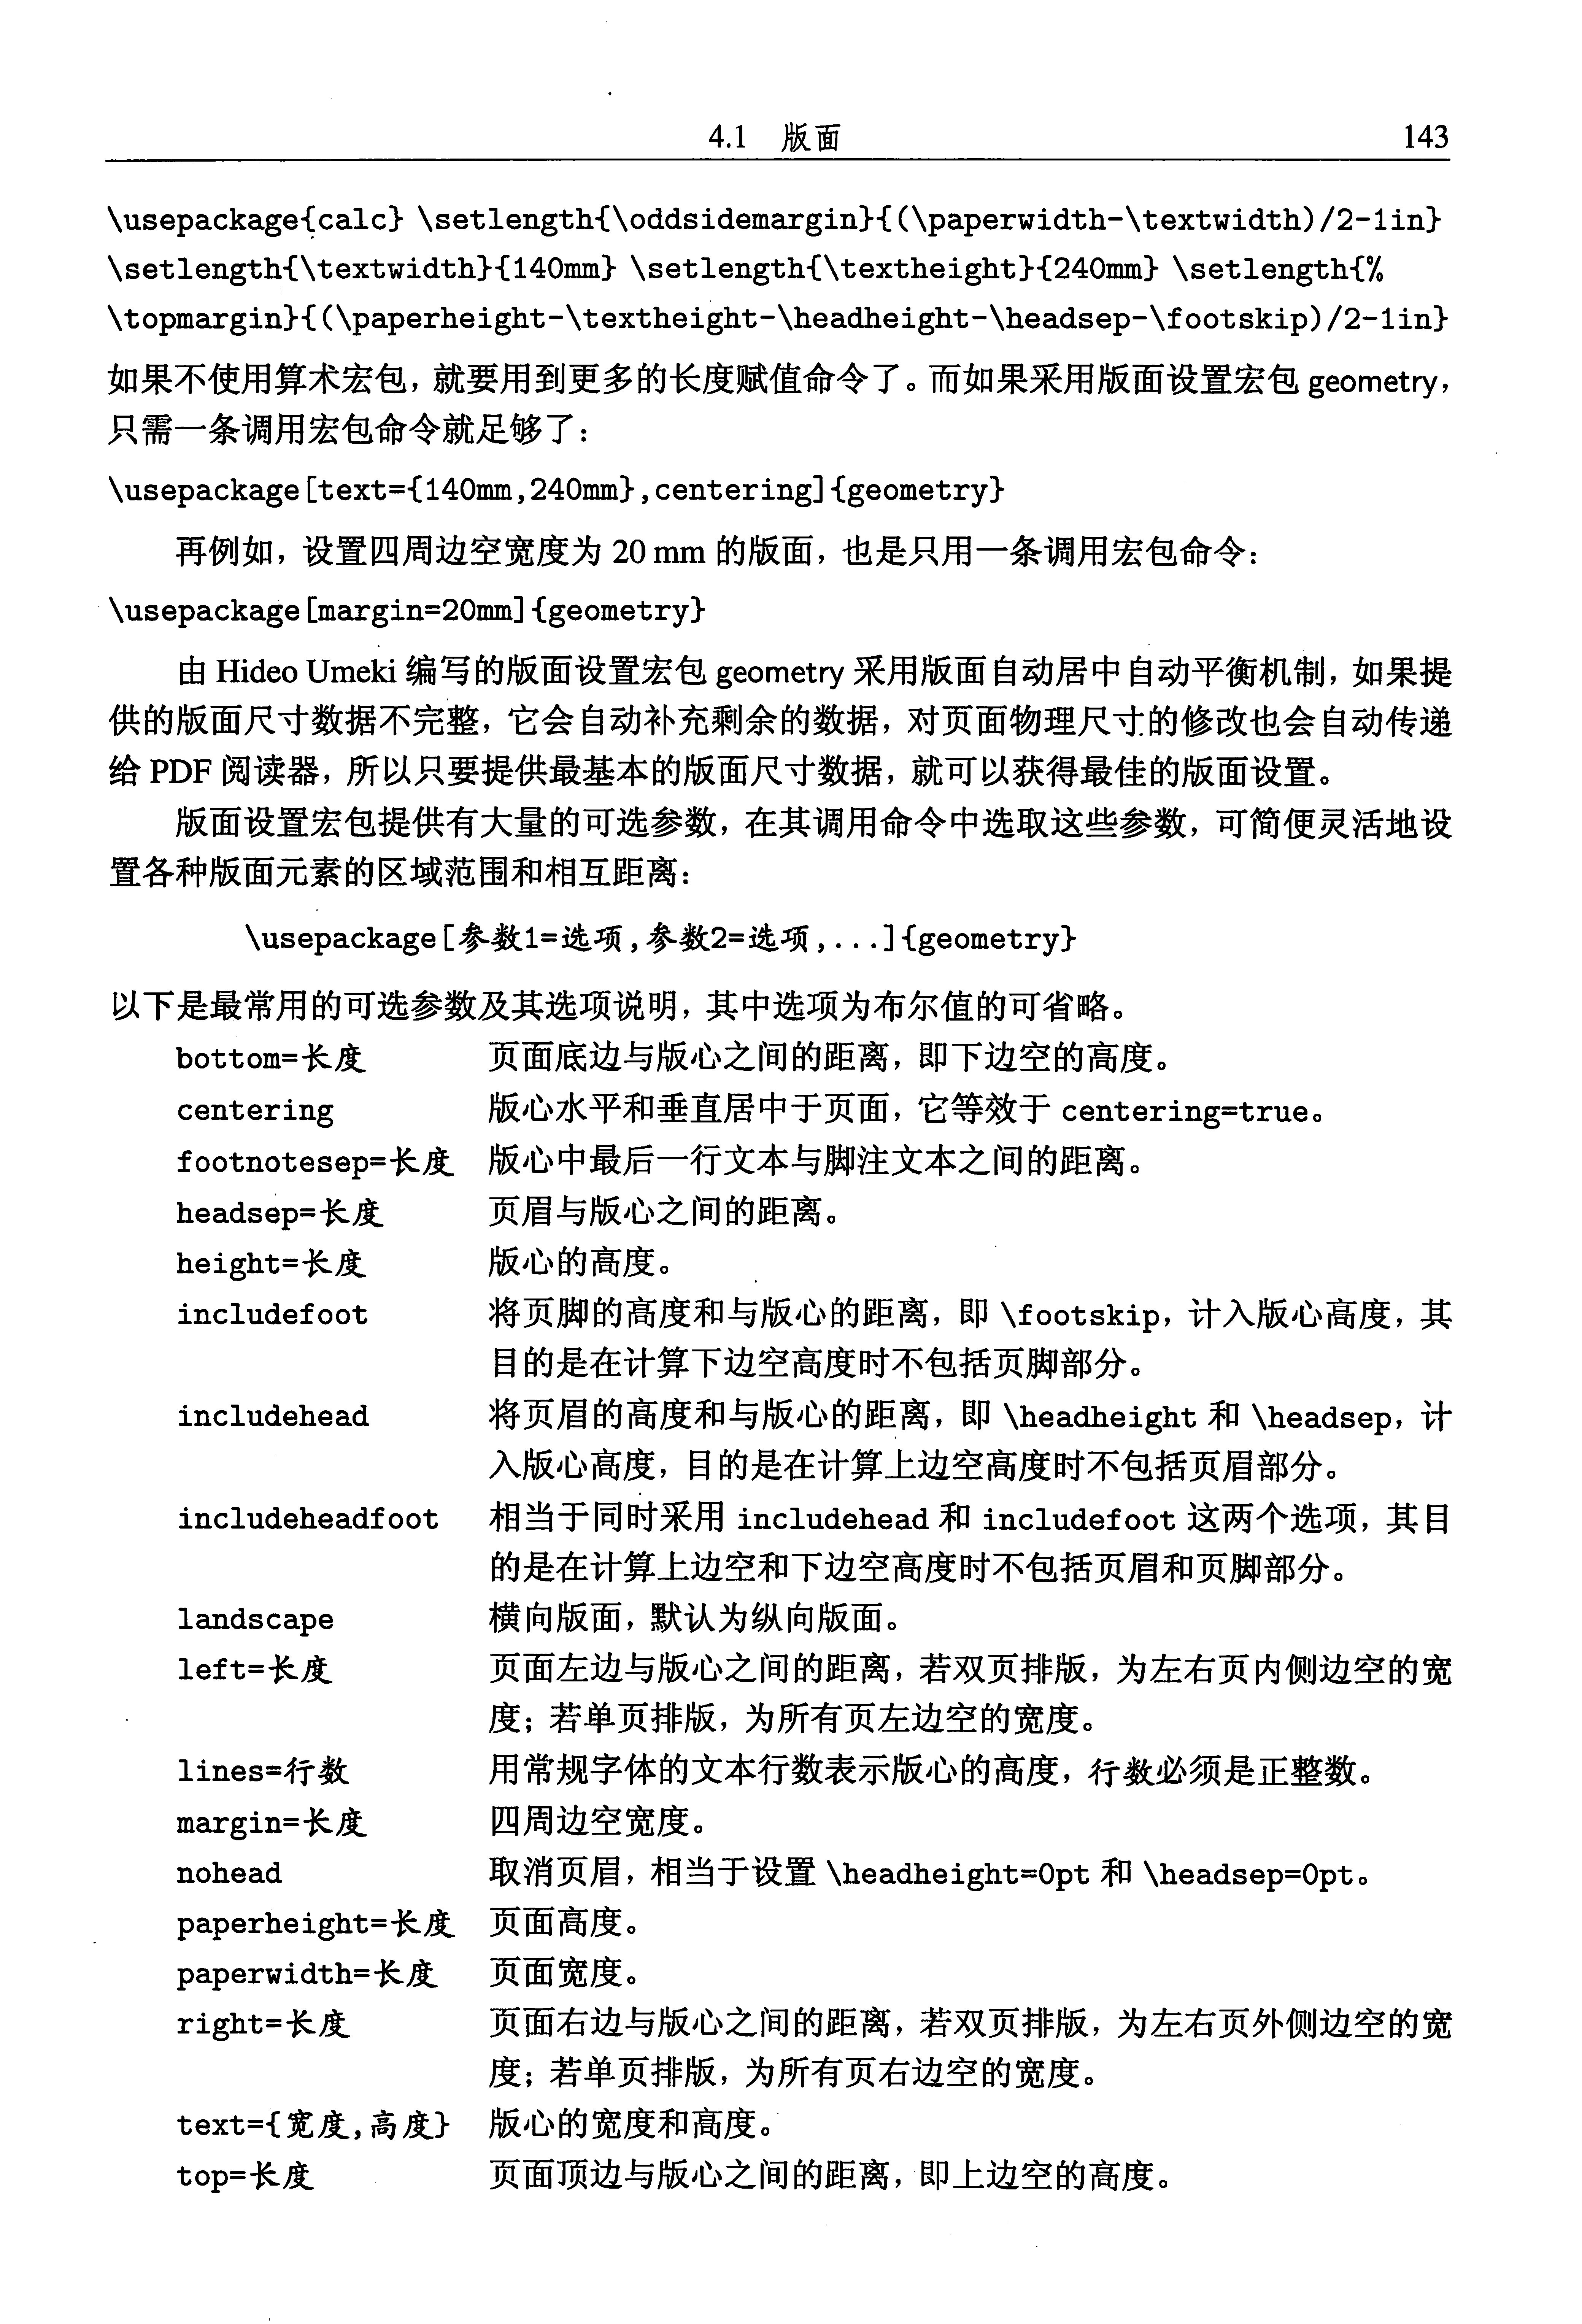
\includegraphics{figures/版面.jpg}
      \caption{版面}
\end{figure*}

\begin{figure*}
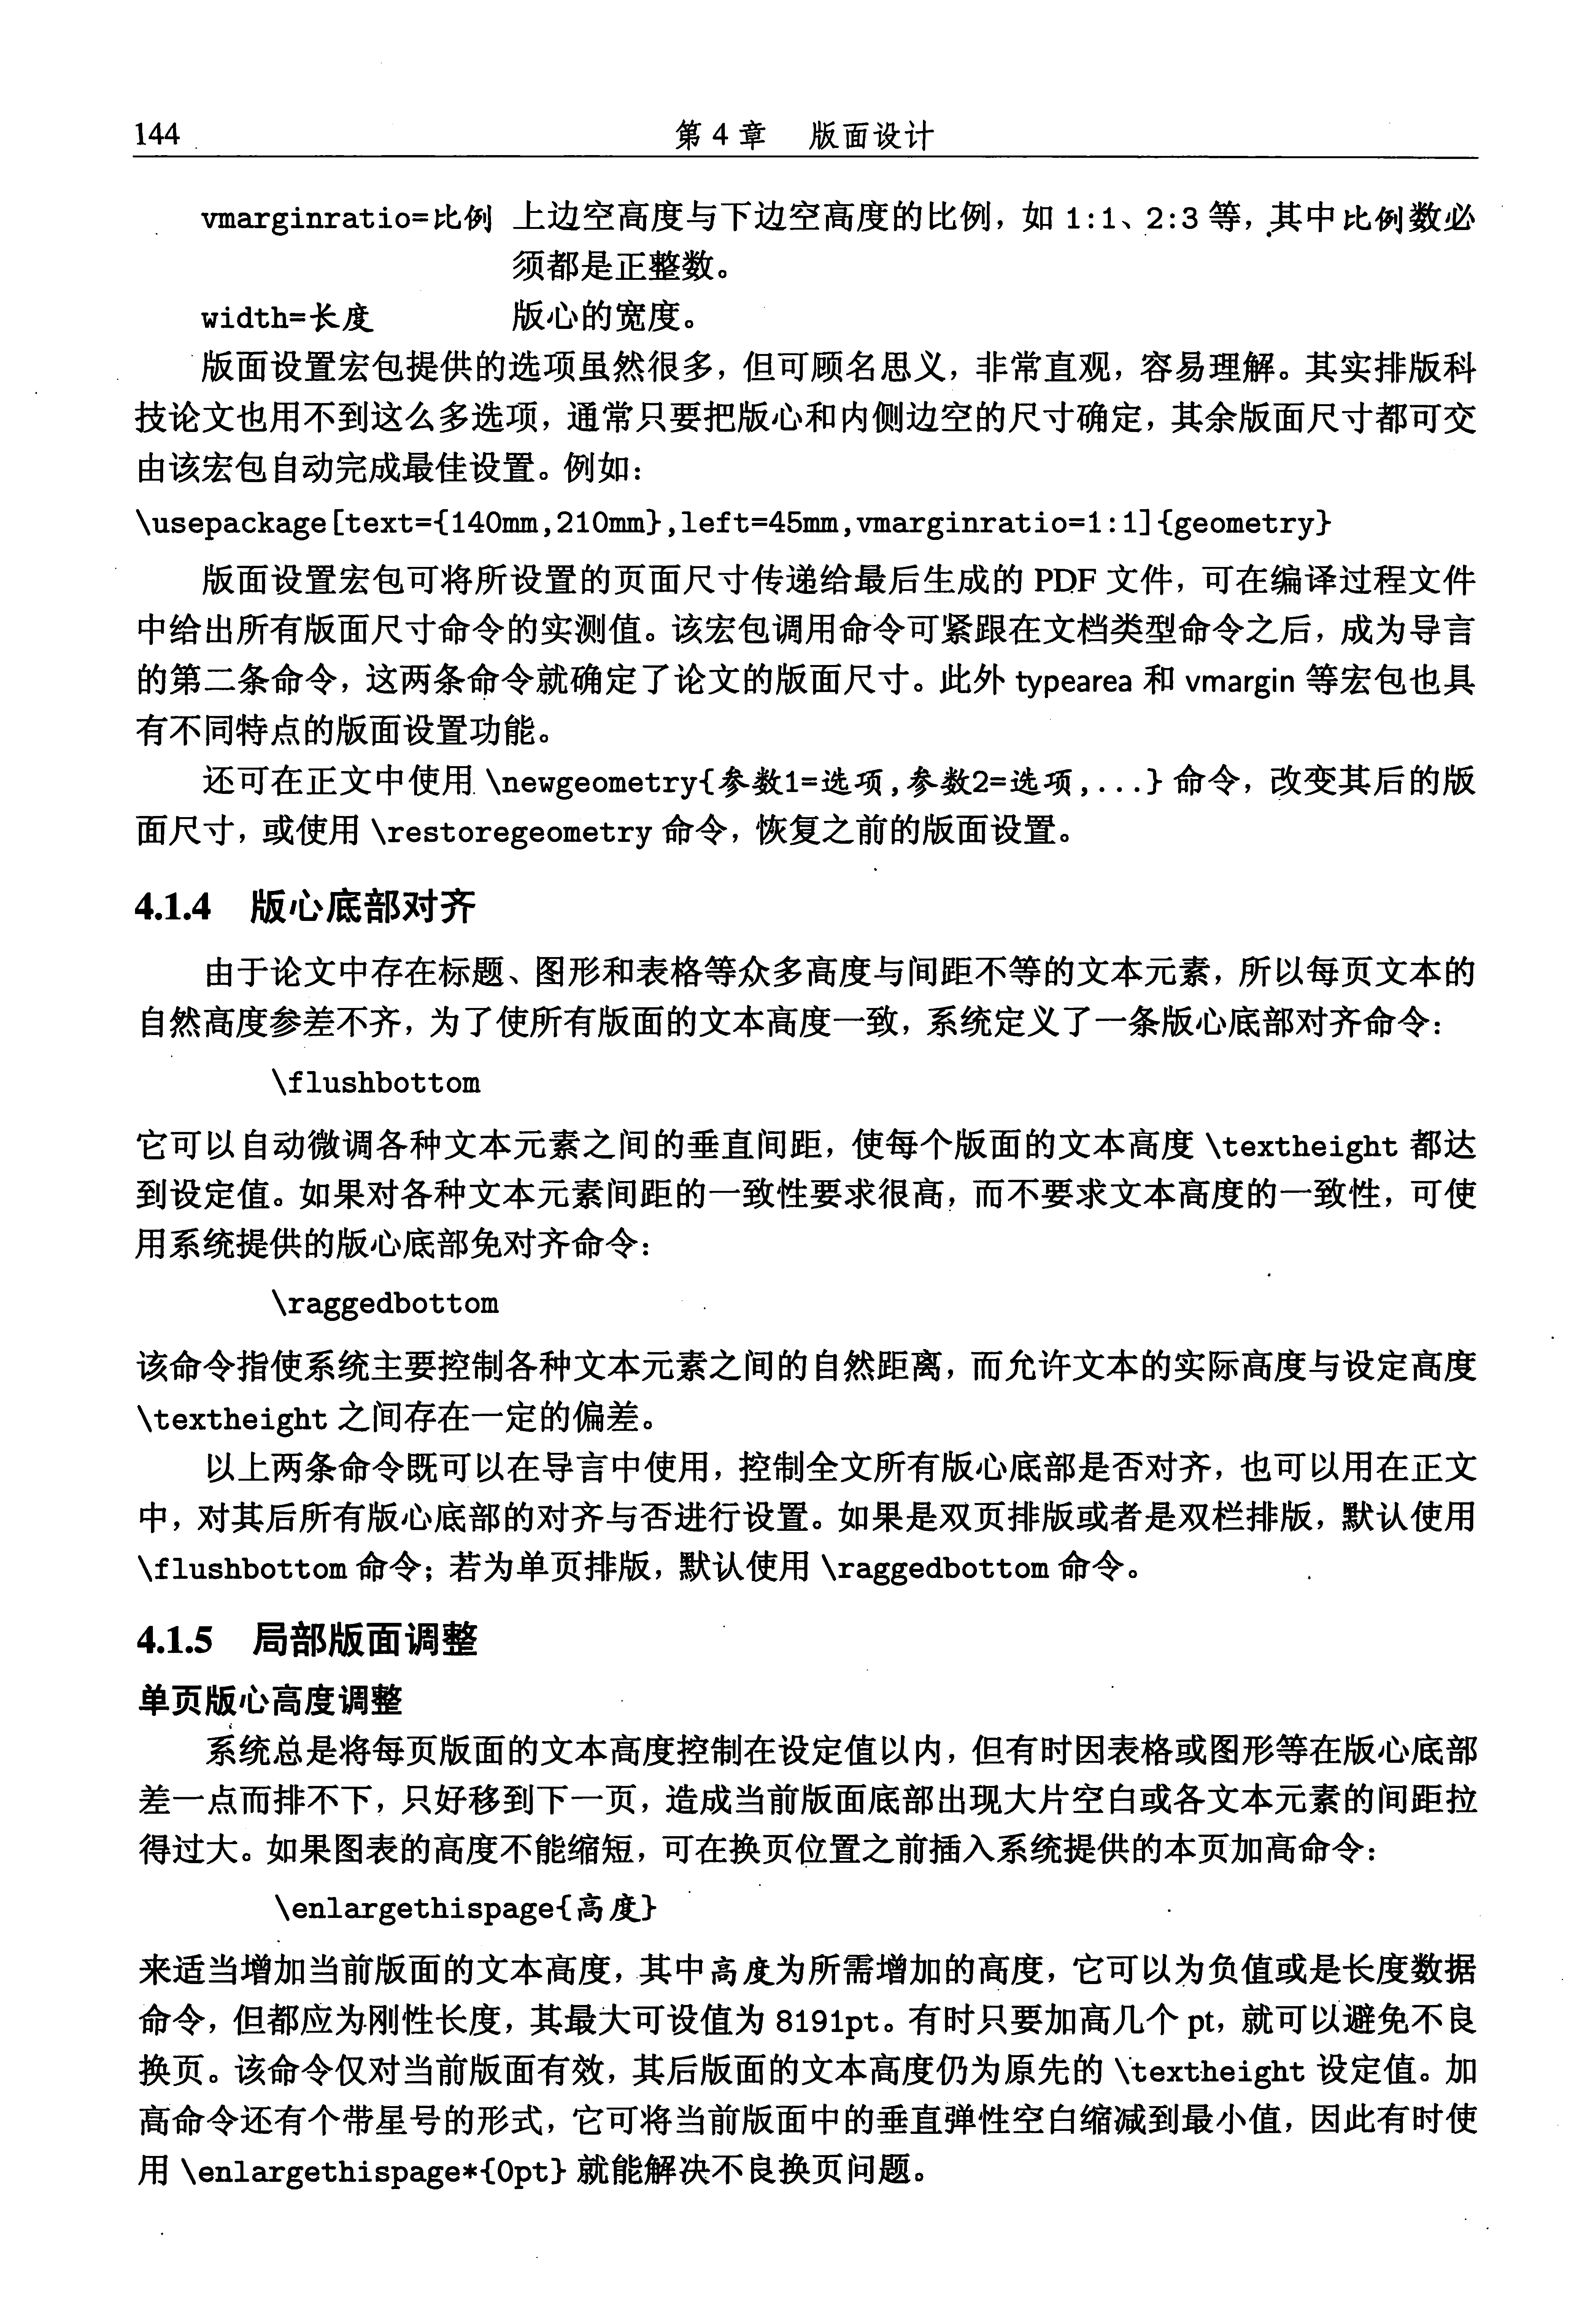
\includegraphics{figures/版面设计.jpg}
      \caption{版面设计}
\end{figure*}

\begin{figure*}
	 includegraphics{figures/字体设计.jpg} 
	 caption{字体设计} 
\end{figure*}


\chapter{Lyx}

\subsection{Setting up LyX to work with XeTeX}

\begin{itemize}
\item check in the menu \textcolor{red}{Document $>$ Settings$>$ Fonts} the option \textcolor{red}{Use non-TeX fonts (via XeTeX/LuaTeX)}. Then you can immediately use the menu \textcolor{red}{View $>$ PDF (XeTeX)}.
\item  Using OpenType fonts (otf) in XeTeX math mode (LyX 2.1)...
\end{itemize}

\paragraph{Setting up XeTeX for CJK scripts}

If you follow the instructions below you can just go ahead and use CJK characters like 猫 into your document (this one means 'cat'). Only CJK characters will use a CJK font and everything else will remain untouched.
Download the xeCJK package from \url{http://www.ctan.org/login/auth}, if it is not yet installed (it should be included in TeXLive and MikTeX).
Add the following lines to Document \textrightarrow Settings \textrightarrow LaTeX Preamble:

\begin{verbatim}
\usepackage{xeCJK}
\setCJKmainfont{Sazanami Mincho}
\end{verbatim}


The detail please see web \url{https://wiki.lyx.org/LyX/XeTeX}

\subsection{LyX + LaTeX}

有些时候Lyx Export的Latex代码不可以直接被Latex编译;同样在Lyx使用Latex代码也会出错,如"input{**.tex}"。为此可以采用如下方法\footnote{1.Lyx使用的是同样的模板;2.Latex的main.tex文件可能需要加载package}:

\begin{itemize}
  \item 在Lyx中写好内容,然后Export Xelatex文件 "name.tex"
  \item 打开“name.tex”文件,删除开头和结尾,只保留主题内容
  \item 此时的”name.tex“ 文件可以被Latex 和 Lyx调用
\end{itemize}


\subsection{input “nameoflayout.layput” into the lyx  and “nameofclass.cls” into latex}

input “nameofclass.cls” into latex\\
Find the location of class
- sudo find / -name revtex4\\
/usr/local/texlive/2016/texmf-dist/tex/latex/

- sudo mv iopart /usr/local/texlive/2016/texmf-dist/tex/latex/

- sudo mktexlsr

input “nameoflayout.layout” into lyx\\
Find the location of layout\\
- sudo find / -name layouts\\
- /Applications/LyX.app/Contents/Resources/layouts\\
\vspace{5mm}

For LyX to see and use the new files, you will need to run Tools > Reconfigure.
Go to Document > Settings > Document Class.  Then from the drop down menu, select “name”.\\
\vspace{5mm}

Note:
\begin{itemize}
  \item There are three file names: nameofclass, nameoflayout and nameforducumentsetting
  \item \textbackslash DeclareLaTeXClass[“nameofclass”]{“namefordocumentsettting”}
  \item In this example, namefordocumentsettting is the name of the LaTeX document class (nameoflcass.cls) and the information in curly brackets is a description which will make it easier to find in the LyX document settings pane.
\end{itemize}

useful web: \url{http://www.oak-tree.us/blog/index.php/2009/11/02/custom-lyx-nih}






Preprocessor directives, like $\#$include statements, simply end at the end of the line and never require semicolons. The beginning of a function, like int main(), is not a complete statement, so you don’t place a semicolon there either. 


% Preview source code for paragraph 0

int main() This marks the beginning of a function. A function can
be thought of as a group of one or more programming statements that
collectively has a name. The name of this function is main, and the
set of parentheses that follows the name indicate that it is a function.
The word int stands for \textquotedblleft integer.\textquotedblright{}
It indicates that the function sends an integer value back to the
operating system when it is finished executing. 

% Preview source code for paragraph 0

\chapter{Tools}
\section{sublime}

set the package $sublime tex \rightarrow preferences \rightarrow package setting$

Sublime Text 使用技巧
。

Sublime快捷键 : \url{https://www.zhihu.com/question/24896283?rf=19976788}

\begin{verbatim}

备注:具体符号对应的按键

⌘Command key
⌃Control key
⌥Option key
⇧Shift Key
为了方便大家记忆,将快捷键分成了8个类型, 分别为

Edit(编辑)
Selection(光标选中)
Find(查找)
View(视图)
Go to(跳转)
Project(工程)
General(通用)
Tabs(标签)
_______________________________________________________
Edit(编辑)
command + [ : 向左缩进 | Left indent
command + ] : 向右缩进 | Right Indent
command + control + ↑ : 与上一行互换(超实用!)| Swap line up
command + control + ↓ : 与下一行互换(超实用!)| Swap line down
command + ← : 去往行的开头 | Beginning of line
command + → : 去往行末尾 | End of line
________________________________________________________
Selection(光标选中)
command + D : 选中相同的词 | Expand selection to words
command + control + G : 多重文本光标选中(再也不用⌘ D一个一个的找啦)| Expand all selection to words
________________________________________
Go to(跳转/定位)
command + P : 跳转文件(很方便)| Go to anything
___________________________________________
Project(工程)
command + control + P : 在保存过的工程中切换,随意变换工程环境|Switch project window

__________________________________________
General(通用)
command + shift + P 打开命令行| Command prompt


\end{verbatim}




\section{git and github}\footnote{\url{https://git-scm.com/book/zh/v2/Git-基础-远程仓库的使用}}

\begin{verbatim}

$ git init
该命令将创建一个名为 .git 的子目录,这个子目录含有你初始化的 
Git 仓库中所有的必须文件,这些文件是 Git 仓库的骨干。

$ git add *.c
$ git add LICENSE
$ git commit -m 'initial project version'

克隆现有的仓库:
$ git clone https://github.com/schacon/ticgit

查看已暂存和未暂存的修改
如果 git status 命令的输出对于你来说过于模糊,你想知道具体修改了什么地方,
可以用 git diff 命令。此命令比较的是工作目录中当前文件和暂存区域快照之间的差异,
 也就是修改之后还没有暂存起来的变化内容。若要查看已暂存的将要添加到下次
 提交里的内容,可以用 git diff --cached 命令。(
 Git 1.6.1 及更高版本还允许使用 git diff --staged,效果是相同的,但更好记些。)

$ git diff --staged
diff --git a/README b/README
new file mode 100644
index 0000000..03902a1
--- /dev/null
+++ b/README
@@ -0,0 +1 @@
+My Project

提交更新
现在的暂存区域已经准备妥当可以提交了。 在此之前,请一定要确认还有什么修改过的
或新建的文件还没有 git add 过,否则提交的时候不会记录这些还没暂存起来的变化。 
这些修改过的文件只保留在本地磁盘。 所以,每次准备提交前,先用 git status 看下,
是不是都已暂存起来了, 然后再运行提交命令 git commit:


移除文件
要从 Git 中移除某个文件,就必须要从已跟踪文件清单中移除(确切地说,是从暂存区域移除)
,然后提交。 可以用 git rm 命令完成此项工作,并连带从工作目录中删除指定的文件,
这样以后就不会出现在未跟踪文件清单中了。

另外一种情况是,我们想把文件从 Git 仓库中删除(亦即从暂存区域移除),但仍然希望保留
在当前工作目录中。 换句话说,你想让文件保留在磁盘,但是并不想让 Git 继续跟踪。 当你
忘记添加 .gitignore 文件,不小心把一个很大的日志文件或一堆 .a 这样的编译生成文件添加
到暂存区时,这一做法尤其有用。 为达到这一目的,使用 --cached 选项:

$ git rm --cached README
git rm 命令后面可以列出文件或者目录的名字,也可以使用 glob 模式。 比方说:

$ git rm log/\*.log
注意到星号 * 之前的反斜杠 \, 因为 Git 有它自己的文件模式扩展匹配方式,所以我们不用 
shell 来帮忙展开。 此命令删除 log/ 目录下扩展名为 .log 的所有文件。 类似的比如:

$ git rm \*~
该命令为删除以 ~ 结尾的所有文件。



$ git remote -v
origin	https://github.com/schacon/ticgit (fetch)
origin	https://github.com/schacon/ticgit (push)

$ git remote add pb https://github.com/paulboone/ticgit
$ git remote -v
origin	https://github.com/schacon/ticgit (fetch)
origin	https://github.com/schacon/ticgit (push)
pb	https://github.com/paulboone/ticgit (fetch)
pb	https://github.com/paulboone/ticgit (push)

现在你可以在命令行中使用字符串 pb 来代替整个 URL。
 例如,如果你想拉取 Paul 的仓库中有但你没有的信息,可以运行 git fetch pb:

$ git fetch pb

推送到远程仓库
当你想分享你的项目时,必须将其推送到上游。 这个命令很简单:
git push [remote-name] [branch-name]。 当你想要将 master 分支推送到 origin 服务器时
(再次说明,克隆时通常会自动帮你设置好那两个名字),那么运行这个命令就可以将你所做的备份到服务器:

$ git push origin master

\end{verbatim}









\chapter{西方哲学}

\section{第一时期:自然秩序}

最早从哲学分离出来的,应该是医学。

毕德格拉斯区分了三中不同生活,他说,来到奥林匹克赛会的有三种人
\begin{itemize}
\item 最低级的是做买卖的人,他们为牟利而来
\item 参加比赛的人,他们为荣誉而来
\item  最好的是观众,他们对正在发生的事情加以思考 \footnote{"观看"与希腊词“理论”是一个意思}
\end{itemize}

他们认为音乐对某些神经错乱颇有疗效,且发现了把弦截成一半,会得到一个高八度的音,“这使得他们认为整个世界就是一个音节,一个数目” \footnote{亚里士多德说的}。

毕德格拉斯定理就是中国的勾股定理。

巴门尼德明确的强调,事物的现象并没有向我们展示实在的构成物质,此思想在柏拉图的哲学中产生了决定性的作用。柏拉图提出真理的理智世界和意见的可见世界之间的区别。

芝诺作为巴门尼德的学生,举例说明了这一点:一粒米种子扔在地上是不会发出声响的,但是如果我们把半蒲式耳种子倒在地上,就会有声音了。芝诺由此得出,我们的感官欺骗的了我们,因此想要到达事物的真理,思想之路要比感觉之路更可靠。

NOTE:


人类最直观,最迫切的一个问题的,我想应该是死亡。正因为我们对死亡的畏惧以及无法解释才使得最开始的祭祀由社会的最高权力机构实施(权力者应该是智力上等人者)。为何哲学在最开始的时候没有涉及到这个问题,这是我很疑惑。思考自热秩序的前提是我们能够将人与自然划一条比较清晰的界限,只有这样才能避开自己,更多的谈及自然。那么也就是说,其实哲学在一开始就在研究人本身。

或许哲学家将这部分留给了巫师,不过这个答案不是很令人满意。


\section{智者派和苏格拉底}

第一批哲学家关注的是自然,而智者派和苏格拉底则讲哲学的问题转到了对人类基本伦理问题的研究\footnote{现在的情况正好相反,人类伦理问题止步不前反倒是自然哲学大步前进}。这一转向可以在下述事实中得到部分解释:前哲学家之间没有能达到任何一种统一的宇宙概念,哲学家在此止步不前。同时此种争论导致了一种怀疑主义的倾向:人类理性是否有能力发现宇宙真理?“我们有没有可能发现普遍真理?”成为了一个新的方向。\footnote{《西方哲学》第二章导言}

三个异乡来的三个智者普罗泰戈拉、高尔基亚、塞拉西马柯(他们自己给自己加上“智者”),他们对雅典娜的人的思想和习俗进行了一番新的审视,提出了一些追根究底的问题,是的雅典娜人不得不考虑自己观念和习俗是基于真理还是仅仅基于惯常的行为习惯。智者派还推动了希腊社会由贵族政体向民主政体的转变。他们把真理看作是一种相对的东西,因此他们利用巧言善辩混淆对错,把不正义的事情说的好像公平合理。将青年从好端端的家庭带走,引导他们去从事要摧毁传统宗教与伦理观点的批判分析。他们的形象已经不同于早期哲学家那种不带任何经济考虑而从事哲学的公正无私的思想家形象。苏格拉底曾在智者门下学习,可是因为穷,他只上的起他们提供的“短期课程”\footnote{让他们描述的有一点儿像如今那些受过高等教育但是专门利用普通民众的‘紧致’利己主义者,例如某些政治家、律师、商人 ... }。

普罗泰戈拉名句:“人是万物的尺度,是存在者的尺度,也是不存在者的尺度。”。 他的相对主义严重打击了人们对有可能大仙真知的信心,也招致了苏格拉底和柏拉图的严厉批评。











































\chapter{install owncloud on ubuntu}
This note is based on the web\footnote{\url{https://ittutorials.net/linux/owncloud/installing-owncloud-in-ubuntu/}}, which shown the almost all steps, but with diffrent version of owncloud and ubuntu, so we need to make some modulation. 

The latest release of ownCloud at the time of this writing is 9.1.0 and the latest Ubuntu LTS release is Ubuntu 16.04 desktop so this tutorial will be based in these two.

\subsection{Update server and set it with a static IP address}

Make sure the server is fully patched. Type \textcolor{red}{sudo apt-get update upgrade} on terminal, then type \textcolor{red}{sudo apt-get dist-upgrade}  reboot the server after all patches have been installed. After the server comes back from the reboot, make sure its set with a static IP.  To see the the server current IP configuration type this on terminal: \textcolor{red}{sudo nano /etc/network/interfaces} and you should get this:

\begin{verbatim}

# interfaces(5) file used by ifup(8) and ifdown(8)

# The loopback network interface
auto lo
iface lo inet loopback


# The primary network interface

auto wlp2s0
iface wlp2s0 inet static

address 192.168.1.10
netmask 255.255.255.0
gateway 192.168.1.1
dns-nameservers 8.8.8.8 8.8.4.4
\end{verbatim}
\footnote{1:address 192.168.1.10 is the IP you use to lauch the owncloud// 2:gateway 192.168.1.1 is the fix, which you shoud set the same with your Ruter}

Save the file by pressing the Ctrl + X keys on your keyboard, and then restart the network service by typing this on terminal: \textcolor{red}{sudo /etc/init.d/networking restart}

\subsection{Installing Apache,PHP and MySQL}

The easiest way to install the LAMP stack at once in Ubuntu is using the Tasksel script. On your terminal type : \textcolor{red}{sudo apt-get install tasksel} and then type \textcolor{red}{sudo tasksel install lamp-server} this will install the basic LAMP stack server for you. Enter a MySQL server password when prompted. After the installation is complete, type the IP address of your server in a browser and you should see the page which title is Apache2 Ubuntu Default Page.

You should probably start with sudo -i so you don’t have to put “sudo” in front of all the following commands or keep re-typing your password. This is a long post but you can easily have everything set up in under 30 minutes. Let’s get everything installed:\footnote{this part is important, please see the detail in web\url{https://www.tombrossman.com/blog/2016/install-owncloud-9-on-ubuntu-16.04/}}

\textcolor{red}{sudo -i apt install apache2 mariadb-server php7.0 php7.0-common libapache2-mod-php7.0 php7.0-gd php-xml-parser php7.0-json php7.0-curl php7.0-bz2 php7.0-zip php7.0-mcrypt php7.0-mysql memcached php-memcached php-redis redis-server}



\subsection{Change PHP max upload limit}

PHP only allows 2MB files upload by default. I assume you will be uploading bigger files to your ownCloud server, so we need to increase the upload size in the php.ini file. To do that, type \textcolor{red}{sudo nano /etc/php5/apache2/php.ini} and search for \textcolor{blue}{upload\_max\_filesize} and for \textcolor{blue}{post\_max\_size} on the file and change both numbers to whatever you need.

Reload apache. \textcolor{red}{Sudo service apache2 reload} 


\subsection{Create the Database}
This part I cannot following the original web page, so I find another way, see web \url{https://www.howtoforge.com/how-to-install-owncloud-7-on-ubuntu-14.04}

login to MySQL and create the database. type \textcolor{red}{mysql –u root –p}

\begin{verbatim}
CREATE DATABASE owncloud;

GRANT ALL ON owncloud.* to 'owncloud'@'localhost' IDENTIFIED BY 'database\_password';

exit;
\end{verbatim}

\subsection{Install ownCloud}

Grab the latest release from the ownCloud website. At the time of this writing, version 9.1 is the latest release. To download it directly from the server, switch to the \textcolor{red}{cd /opt/} directory, and type this command in terminal: \textcolor{red}{sudo wget https://download.owncloud.org/community/owncloud-9.1.0.zip}

\begin{itemize}
        \item Unzip the archive with this command: sudo unzip owncloud-9.0.0.zip
        \item Move the ownCloud files to the the WWW web directory: sudo mv /opt/owncloud /var/www/
        \item Make apache the owner of this directory : sudo chown –R www-data:www-data /var/www/owncloud/
        \item Change your apache virtual host to point to this ownCloud directory:  sudo nano /etc/apache2/sites-available/000-default.conf change the DocumentRoot to /var/www/owncloud/
\end{itemize}


Type in the IP address\footnote{192.168.1.10 in my case} of your server in your preferred browser and you should get a webpage which shows a general web of owncloud but needs more modules. In my case, I need install php7.0-md and multi.



 Install them by typing this on terminal \textcolor{red}{sudo apt-get install php5-md} and \textcolor{red}{sudo apt-get install multi} reload apache again:  \textcolor{red}{sudo service apache2 reload} and the ownCloud wizard shouldn’t complain now.


\textcolor{blue}{Username Password} is the username and password you use to landing the owncloud. 

In the lower tab below the MySQL/MariaDB give the entry of the \textcolor{blue}{username=owncloud password=database\_password databasename=owncloud}

Then press \textcolor{blue}{Finish} setup.



\chapter{Blender}

blender could convert the movie, such as format like '.mp4', to pictures squence, like '.png'.

\begin{itemize}
\item Blender does not support the gif format.
\item For a list of supported formats see \url{https://www.blender.org/manual/data_system/files/media/image_formats.html#image-formats}
\end{itemize}


Two way to choose the object

\begin{itemize}
\item  bpy.data.objects["Cube"]
\item bpy.context.object \footnote{While it’s useful to be able to access data directly by name or as a list, it’s more common to op‐ erate on the user’s selection. The context is always available from bpy.context and can be used to get the active object, scene, tool settings along with many other attributes.

Note that the context is read-only. These values cannot be modified directly, though they may be changed by running API functions or by using the data API.
So bpy.context.object = obj will raise an error.
But bpy.context.scene.objects.active = obj will work as expected.
}
\end{itemize}

Animation

There are 2 ways to add keyframes through Python.
The first is through key properties directly, which is similar to inserting a keyframe from the but‐ ton as a user. You can also manually create the curves and keyframe data, then set the path to the property. Here are examples of both methods.
Both examples insert a keyframe on the active object’s Z axis.


Simple example:

\begin{verbatim}
Using Low-Level Functions:
obj = bpy.context.object
obj.location[2] = 0.0
obj.keyframe_insert(data_path="location", frame=10.0, index=2)
obj.location[2] = 1.0
obj.keyframe_insert(data_path="location", frame=20.0, index=2)
\end{verbatim}



Using Low-Level Functions:

\begin{verbatim}
obj = bpy.context.object
obj.animation_data_create()
obj.animation_data.action = bpy.data.actions.new(name="MyAction")
fcu_z = obj.animation_data.action.fcurves.new(data_path="location", index=2)
fcu_z.keyframe_points.add(2)
fcu_z.keyframe_points[0].co = 10.0, 0.0
fcu_z.keyframe_points[1].co = 20.0, 1.0
\end{verbatim}


\section{The python file for moving object}
\begin{verbatim}
import bpy  
from math import sin
from mathutils import Vector

# useful shortcut
scene = bpy.context.scene

# this shows you all objects in scene
scene.objects.keys()

# when you start default Blender project, first object in scene is a Cube
kostka = scene.objects[0]

# you can change location of object simply by setting the values
kostka.location = (1,2,0)

# same with rotation
kostka.rotation_euler = (45,0,0)

# this will make object cease from current scene
scene.objects.unlink(kostka)

# clear everything for now
scene.camera = None  
for obj in scene.objects:  
    scene.objects.unlink(obj)

# create sphere and make it smooth
bpy.ops.mesh.primitive_uv_sphere_add(location = (2,1,2), size=0.5)  
bpy.ops.object.shade_smooth()  
kule = bpy.context.object

# create new cube
bpy.ops.mesh.primitive_cube_add(location = (-2,1,2))  
kostka = bpy.context.object

# create plane 
bpy.ops.mesh.primitive_plane_add(location=(0,0,0))  
plane = bpy.context.object  
plane.dimensions = (20,20,0)

# for every object add material - here represented just as color
for col, ob in zip([(1, 0, 0), (0,1,0), (0,0,1)], [kule, kostka, plane]):  
    mat = bpy.data.materials.new("mat_" + str(ob.name))
    mat.diffuse_color = col
    ob.data.materials.append(mat)

# now add some light
lamp_data = bpy.data.lamps.new(name="lampa", type='POINT')  
lamp_object = bpy.data.objects.new(name="Lampicka", object_data=lamp_data)  
scene.objects.link(lamp_object)  
lamp_object.location = (0, 0, 12)

# and now set the camera
cam_data = bpy.data.cameras.new(name="cam")  
cam_ob = bpy.data.objects.new(name="Kamerka", object_data=cam_data)  
scene.objects.link(cam_ob)  
cam_ob.location = (-1, -1, 5)  
cam_ob.rotation_euler = (3.14/6,0,-0.3)  
cam = bpy.data.cameras[cam_data.name]  
cam.lens = 10


### animation
# positions = ((0,0,2),(0,1,2),(3,2,1),(3,4,1),(1,2,1))

positions = []
angles = []

end = 500

for i in range(0,end):
    positions.append((i/50., 3*sin(i/5.), 1)) 
    #positions.append((0,0,i))


# start with frame 0
number_of_frame = 0  
bpy.context.scene.frame_end = end

for pozice in positions:

    # now we will describe frame with number $cislo_snimku
    scene.frame_set(number_of_frame)

    # set new location for sphere $kule and new rotation for cube $kostka
    kule.location = pozice
    kule.keyframe_insert(data_path="location", index=-1)


    #kostka.location = pozice
    #kostka.keyframe_insert(data_path="location", index=-1)

    kostka.rotation_euler = pozice
    kostka.keyframe_insert(data_path="rotation_euler", index=-1)

    # move next 10 frames forward - Blender will figure out what to do between this time
    number_of_frame += 1
\end{verbatim}
 


%\chapter{Blender python}

\section{GameLogic Module}

\subsection{expandPath}

\begin{verbatim}
expandPath(include)
Expands the path to include the directory of the blend that was opened.

include:
Type:  string
           "//" = expands path to include the directory of the blend opened.

Note:
You can include subdirectories by using ("//" + "subdir_name\\")

Sample Code

# get the path to the blend directory
mainDir = GameLogic.expandPath("//")

# get path to subdirectory named Sound
soundDirectory = mainDir + "Sound\\"

# get path to scream.wav
screamPath = (soundDirectory + "scream.wav")
\end{verbatim}


\subsection{getAverageFrameRate}

\begin{verbatim}
getAverageFrameRate()

Returns the estimated frames per second

Return type:   float
Sample Code

# get the FPS
fps = GameLogic.getAverageFrameRate()
\end{verbatim}

\subsection{getBlendFileList}
\begin{verbatim}
getBlendFileList(dirPath)

Returns a list of the blend files in a directory.

Return type:  List [ string ]

dirPath:
Type:  string

Note:
Works the same as expandPath.

Note:  
Leaving dirPath blank -- ie. GameLogic.getBlendFileList() -- returns a list of the blend files in the same directory as the open blend.

Sample Code
# get a list of the blends in the same directory as open blend
blendList = GameLogic.getBlendFileList("//")

# get a list of the blends in subDirectory Data
dataBlendList = GameLogic.getBlendFileList("//" + "Data\\")

# get list of the blends in C:\MyGames\Blender
gameBlends = GameLogic.getBlendFileList("C:\\MyGames\\Blender\\")
\end{verbatim}

\subsection{getCurrentController}
\begin{verbatim}
getCurrentController()
Returns the controller logic brick that this python script is attached to.

Return type:
SCA_PythonController
Sample Code

# get the controller
controller = GameLogic.getCurrentController()
\end{verbatim}


\subsection{getCurrentScene}
\begin{verbatim}
getCurrentScene()

Returns the current scene

Return type:
KX_Scene
Sample Code

# get current scene
scene = GameLogic.getCurrentScene()
\end{verbatim}


\subsection{getLogicTicRate}
\begin{verbatim}

getLogicTicRate()

Returns how many times per second the logic bricks sensors are being checked/fired.  

The default is 60 times per second (60 Hz)

Return type:
float number
Sample Code

# get the logic tic rate
ticRate = GameLogic.getLogicTicRate()
\end{verbatim}

\subsection{getMaxLogicFrame}

\begin{verbatim}
getMaxLogicFrame()

Returns the number of logic frames executed per render frame.

Return type:  integer

Range:  1 - 5

Note:
The default is 5 logic frames executed per render frame.
Sample Code

# get the max logic frame 
maxLogic = GameLogic.getMaxLogicFrame()
\end{verbatim}

\subsection{getPhysicsTicRate}

\begin{verbatim}
getPhysicsTicRate()

Returns how many times per second the scene's physics are being updated.  

Return type:  float 

Note:
Always returns 0.0
Sample Code

# get the physics tic rate
ticRate = GameLogic.getPhysicsTicRate()
\end{verbatim}

\subsection{getRandomFloat}

\begin{verbatim}
getRandomFloat()

Returns a random float number between 0.0 and 1.0

Return type:  float
Sample Code

# get a random number to use as a seed
seed = GameLogic.getRandomFloat()
\end{verbatim}

\subsection{getSceneList}
\begin{verbatim}
getSceneList()

Returns a list of the active scenes

Returns: list[ KX_Scene ]
Sample Code

activeScenes = GameLogic.getSceneList()
\end{verbatim}

\subsection{getSpectrum}
\begin{verbatim}
getSpectrum()

Returns a 512 point list from the sound card

This is from the official documentation

Returns: list[float]

len(getSpectrum()) == 512

Note:
This only works if the fmod sound driver is being used.
Sample Code

None
\end{verbatim}

\subsection{PrintGLInfo}
\begin{verbatim}
PrintGLInfo()

Prints the following information about OpenGL extensions to the Blender 3D console window.

Supported Extensions...
GL_ARB_shader_objects supported?
GL_ARB_vertex_objects supported?
--------- Details -----------
Max uniform components
Max varying floats
Max vertex texture units
Max combined texture units

GL_ARB_fragment_shader supported?
---------- Details -----------
Max uniform components

GL_ARB texture_cube_map supported?
----------- Details ----------
Max cubemap size

GL_ARB_multitexture supported?
----------- Details -----------
Max texture units available

GL_ARB_texture_env_combine supported?
Sample Code

#Print info about OpenGL extensions
GameLogic.PrintGLInfo()
\end{verbatim}


\subsection{sendMessage}
\begin{verbatim}
sendMessage(subject, body, to, from)

Sends a message to a sensor 

subject:
The subject of the message
Type:  String
body:
The body of the message (optional)
Type:  String
to:
The name of the object to send the message to (optional)
Type:  String
from: 
The name of the object that the message is coming from (optional)
Type:  String
Sample Code

# send message to Cube
GameLogic.sendMessage("Rotate", "none", "OBCube", "OBSuzanne")
\end{verbatim}

\subsection{setGravity}
\begin{verbatim}
setGravity(gravity)

Sets the world gravity using the world x, y and z axis.

gravity:
Type:  list [ x, y, z]
Sample Code

# set the gravity to 10 (-z axis direction)
GameLogic.setGravity([ 0.0, 0.0, -10.0])
\end{verbatim}

\subsection{setLogicTicRate}
\begin{verbatim}
setLogicTicRate(ticRate)

Sets how many times per second the logic brick sensors are checked/fired.  

The default is 60 times per second (60 Hz)

ticRate:
Type:  float number
Sample Code

# set the logic tic rate to 100
GameLogic.setLogicTicRate(100.0)
\end{verbatim}

\subsection{setMaxLogicFrame}
\begin{verbatim}
setMaxLogicFrame(logicRate)

Note:
The default is 5 logic frames executed per render frame.

Sets the number of logic frames executed per render frame.

logicRate
Type:  integer

Range:  1 - 5
Sample Code

# set max logic frame to 4
GameLogic.setMaxLogicFrame(4)
\end{verbatim}

\subsection{setMaxPhysicsFrame}
\begin{verbatim}
setMaxPhysicsFrame(physicsRate)

Sets the number of physics frames executed per render frame.

physicsRate
Type:  integer

Range:  1 - 5
Sample Code

# set max physics frame to 4
GameLogic.setMaxPhysicsFrame(4)
\end{verbatim}

\subsection{setPhysicsTicRate}
\begin{verbatim}
setPhysicsTicRate(ticRate)

Sets how many times per second the scene's physics are being updated.  

The default is 60 times per second (60 Hz)

ticRate:
Type:  float number

Note:
Doesn't work
Sample Code

# set the physics tic rate to 120
GameLogic.setPhysicsTicRate(120.0)
\end{verbatim}

\subsection{stopDSP}
\begin{verbatim}
stopDSP()

Stops the sound driver using DSP effects

Note:
This only works if the fmod sound driver is being used.
Sample Code

None
\end{verbatim}


\subsection{globalDict}

\begin{verbatim}
globalDict

Stores/saves the name and values of variables so they can be passed between scenes.

Note:
This is the Blender version of a python dictionary.  

Note:
A dictionary is a python data structure.  Different types (float, integer, string, dictionary, etc) of data can be stored in the same dictionary.
Sample Code

#create a dictionary for player 1 stats
player1_Stats = {  "Health" : 80,
"Armor" : 30,
"Class" : "Cleric"  }
                
#create a dictionary for player 2 stats
player2_Stats = {  "Health" : 60,
"Armor" : 90,
"Class" : "Warrior"  }

# save player 1 and player 2 dictionarys to the globalDict
GameLogic.globalDict["player1"] = player1_Stats 
GameLogic.globalDict["player2"] = player2_Stats

# get player 1 stats from the globalDict
player1_stats = GameLogic.globalDict.get("player1")

# get player 2 stats from the globalDict
player2_stats = GameLogic.globalDict.get("player2")
\end{verbatim}


%\section{Mathutils Module}



\subsection{AngleBetweenVecs}
\begin{verbatim}
AngleBetweenVecs(vec1, vec2)
Returns the angle between two vectors

Return Type:  Angle (in degrees)

vec1:
A 2D or 3D Vector 
vec2:
A 2D or 3D Vector 
Sample Code
# import mathutils
import Mathutils

# create 1st vector 
vec1 = Mathutils.Vector(1.0, 0.0, 0.0)

# create 2nd vector 
vec2 = Mathutils.Vector(0.0, 0.0, 1.0)

# find angle between two
ang = Mathutils.AngleBetweenVecs(vec1, vec2)
\end{verbatim}

\subsection{CrossQuats}
\subsection{CrossVecs}
\subsection{CrossQuats}
\begin{verbatim}
CrossQuats(quat1, quat2)

Return the cross product of two quaternions.

Return Type:  Quaternion

quat1:
Type:  Quaternion 
quat2
Type:  Quaternion 
Sample Code

# import Mathutils
import Mathutils

# create 1st Quaternion 
quat1= Mathutils.Quaternion(1.0, 2.0 ,3.0 ,4.0 )

# create 2nd Quaternion 
quat2= Mathutils.Quaternion(5.0, 6.0 ,7.0 ,8.0 )

# use cross product to create a new Quaternion 
quatCross = Mathutils.CrossQuats(quat1, quat2)
\end{verbatim}

\subsection{DifferenceQuats}
\begin{verbatim}
DifferenceQuats(quat1, quat2)
Returns the rotational difference between the two quaternions. 

Return Type:  Quaternion

quat1:
Type:  Quaternion 
quat2
Type:  Quaternion 
Sample Code
# import Mathutils
import Mathutils

# create 1st Quaternion 
quat1= Mathutils.Quaternion(1.0, 2.0 ,3.0 ,4.0 )

# create 2nd Quaternion 
quat2= Mathutils.Quaternion(5.0, 6.0 ,7.0 ,8.0 )

# get the rotational difference
quatRotDiff = Mathutils.DifferenceQuats(quat1, quat2)
\end{verbatim}

\subsection{DotQuats}
\begin{verbatim}
DotQuats(quat1, quat2)

Returns the scalar product of quaternion muliplication.

Return Type: float

quat1:
Type:  Quaternion 
quat2
Type:  Quaternion 
Sample Code

# import Mathutils
import Mathutils

# create 1st Quaternion 
quat1= Mathutils.Quaternion(1.0, 2.0 ,3.0 ,4.0 )

# create 2nd Quaternion 
quat2= Mathutils.Quaternion(5.0, 6.0 ,7.0 ,8.0 )

# use DotQuats
quatDot = Mathutils.DotQuats(quat1, quat2)
\end{verbatim}

\subsection{DotVecs}
\begin{verbatim}
DotVecs(vec1, vec2)

Returns scalar product of vector muliplication.

Return Type:  float

vec1:
Type:   a 2D, 3D or 4D Vector)
vec2
Type:   a 2D, 3D or 4D Vector)
Sample Code

# import Mathutils
import Mathutils

# create 1st vector 
vec1 = Mathutils.Vector(1.0, 0.0, 0.0)

# create 2nd vector 
vec2 = Mathutils.Vector(0.0, 0.0, 1.0)

# use DotVecs
vecDot = Mathutils.DotVecs(vec1, vec2)
\end{verbatim}


\subsection{Intersect}
\begin{verbatim}
Intersect(vec1, vec2, vec3, ray, orig, clip)
Note:
Returns None if the ray doesn't intersect the triangle.

Returns the intersection between a ray and a triangle, if possible, return None otherwise.

Return Type:  Vector

vec1
Type:  3D Vector  (1st corner of the triangle)
vec2
Type:  3D Vector  (2nd corner of the triangle)
vec3
Type:  3D Vector  (3rd corner of the triangle)
ray
Type:  3D Vector 
   The orientation of the ray. The length of the ray is not used
orig
 Type:  3D Vector
   The origin of the ray.
clip 
Type:  integer 
   0 = don't restrict the intersection to the area of the triangle
 (Use the infinite plane defined by the triangle.)
   1 = restrict to intersection with triangle area
Sample Code
# import Mathutils
import Mathutils

# create 1st vector for 1st corner
vec1 = Mathutils.Vector( 0.0, 0.0, 0.0)

# create 2nd vector for 2nd corner
vec2 = Mathutils.Vector (6.0, 0.0, 0.0)

# create 3rd vector for 3rd corner
vec3 = Mathutils.Vector( 0.0, 0.0, 6.0)

# create ray vector 
ray = Mathutils.Vector( 0.0, 1.0, 0.0)

# create origin vector
orig = Mathutils.Vector(2.0, -2.0, 2.0)

# get intersection for an infinite plane
vecIntersect = Mathutils.Intersect(vec1, vec2, vec3, ray, orig, 0)
\end{verbatim}

\subsection{LineIntersect}
\begin{verbatim}
LineIntersect(vec1, vec2, vec3, vec4)

Note:
Because the lines are evaluated as infinite lines in space, the values returned may not be between the 2 points given for each line.

Returns a tuple with the points on each line respectively closest to the other (when both lines intersect, both vector hold the same value). 

Return Type:  ([Vector], [Vector])

vec1
A 3d vector, one point on the first line
Type:  Vector
vec2 
A 3d vector, another point on the first line
Type:  Vector
vec3
A 3d vector, one point on the second line
Type:  Vector
vec4
A 3d vector, another point on the second line
Type:  Vector
Sample Code

# import Mathutils
import Mathutils

# create 1st vector for 1st point on 1st line
vec1 = Mathutils.Vector(0.0, 0.0, 0.0)

# create 2nd vector for 2nd point on 1st line
vec2 = Mathutils.Vector(5.0, 0.0, 0.0)

# create 1st vector for 1st point on 2nd line
vec3 = Mathutils.Vector(2.0, -2.0, 0.0)

# create 2nd vector for 2nd point on 2nd line
vec4 = Mathutils.Vector(2.0, 2.0, 0.0)

# get line intersect
lineIntersect = Mathutils.LineIntersect(vec1, vec2, vec3, vec4)
\end{verbatim}

\subsection{MidpointVecs}
\begin{verbatim}
MidpointVecs(vec1, vec2)

Returns a vector to the midpoint between two vectors.

Return Type:  Vector

vec1:
Type:   a 2D, 3D or 4D Vector)
vec2
Type:   a 2D, 3D or 4D Vector)
Sample Code

# import Mathutils
import Mathutils

# create 1st vector 
vec1 = Mathutils.Vector(1.0, 0.0, 0.0)

# create 2nd vector 
vec2 = Mathutils.Vector(0.0, 0.0, 1.0)

# use MidpointVecs
vecMid = Mathutils.MidpointVecs(vec1, vec2)
\end{verbatim}

\subsection{OrthoProjectionMatrix}
\begin{verbatim}
OrthoProjectionMatrix(plane, matSize, axis)

Returns a matrix that represents an orthographic projection

Return Type: Matrix

plane
Type:  string
  "x"   = x projection 2D
  "y"   = y projection 2D
  "xy" = xy projection
  "xz" = xz projection
  "yz" = yz projection
  "r"   = arbitrary projection plane
matSize
Type:  integer
  The size of the projection matrix to construct. Can be 2D, 3D, or 4D.
axis  (optional -- The arbitrary axis used with the "R" plane type)
Type: Vector
  Arbitrary perpendicular plane vector.
Sample Code

# import Mathutils
import Mathutils

# create a 2D Matrix
orthoMatrix = Mathutils.OrthoProjectionMatrix("x" , 2)

# create a 3D Matrix
orthoMatrix = Mathutils.OrthoProjectionMatrix("xy" , 3)
\end{verbatim}

\subsection{ProjectVecs}
\begin{verbatim}
ProjectVecs(vec1, vec2)
Returns the parallel projection vector (the projection of vec1 onto vec2).

Return Type:  Vector

vec1:
Type:   a 2D, 3D or 4D Vector)
vec2
Type:   a 2D, 3D or 4D Vector)
Sample Code
# import Mathutils
import Mathutils

# create 1st vector 
vec1 = Mathutils.Vector(1.0, 0.0, 0.0)

# create 2nd vector 
vec2 = Mathutils.Vector(0.0, 0.0, 1.0)

# use ProjectVecs
vecProject= Mathutils.ProjectVecs(vec1, vec2)
\end{verbatim}


\subsection{QuadNormal}
\begin{verbatim}
QuadNormal(vec1, vec2, vec3, vec4)
Returns the normal of the 3D quad defined.

Return Type:  Vector

vec1:
Type:   3D Vector  
    (the 1st vertex of the quad)
vec2
Type:   3D  Vector
    (the 2nd vertex of the quad)
vec3:
Type:   3D Vector  
    (the 3rd vertex of the quad)
vec4
Type:   3D  Vector
    (the 4thvertex of the quad)
Sample Code
# import Mathutils
import Mathutils

# create 1st Vector for the vertex
vec1= Mathutils.Vector(0.0, 0.0, 0.0)

# create 2nd Vector for 2nd vertex
vec2= Mathutils.Vector(1.0, 0.0, 0.0)

# create 3rd Vector for the 3rd vertex
vec3= Mathutils.Vector(1.0, 0.0, 1.0)

# create 4th Vector for 4th vertex
vec4= Mathutils.Vector(0.0, 0.0, 1.0)

# use QuadNormal
quadNormal = Mathutils.QuadNormal(vec1, vec2, vec3, vec4)
\end{verbatim}

\subsection{Rand}
\begin{verbatim}
Rand(low, high)
Return a random number between 0.0 and 1.0

Return Type:  float

low
Type:  float
Range:  0.0 - 1.0
lhigh
Type:  float
Range:  0.0 - 1.0
Sample Code
# import Mathutils
import Mathutils

# create random number between 0.0 and 0.8
randNum = Mathutils.Rand(0.0, 0.8)
\end{verbatim}


\subsection{rotate}
\begin{verbatim}
rotate(angle, axis)

Rotates a euler by a fixed amount of degrees around an axis.

angle  (degrees to rotate)
Type:  float) 
axis   (axis to rotate around)
Type:  string
  "x" or "y" or  "z"
Sample Code

# import Mathutils
import Mathutils

# create a Euler object
euler = Mathutils.Euler(45,0,0)

# rotate euler 90 degrees around the x axis
euler.rotate( 90.0, "x")
\end{verbatim}


\subsection{RotationMatrix}
\begin{verbatim}
RotationMatrix(angle, matSize, axisFlag, axis)

Creates a matrix representing a rotation.

Returns Type:  Matrix

angle  (The angle of rotation desired)
Type:  float) 

matSize  (The size of the rotation matrix to construct. Can be 2x2, 3x3, or 4x4)
Type:  Integer

axisFlag
Type:  string
  "x" = x-axis rotation
  "y" = y-axis rotation
  "z" = z-axis rotation"
  "r" =  arbitrary rotation around vector

axis:  (optional -- The arbitrary axis of rotation used with the "R" axisFlag)
Type=Vector 
Sample Code

# import Mathutils
import Mathutils

# use RotationMatrix
matrixNew = Mathutils.RotationMatrix(90.0, 3, "x")
\end{verbatim}

\subsection{ScaleMatrix}
\begin{verbatim}
ScaleMatrix(factor, matSize, axis)
Creates a matrix representing a scaling.

Return Type:  Matrix

factor
The factor of scaling to apply.
Type:  float 

matSize 
The size of the scale matrix. Can be 2x2, 3x3, or 4x4.
Type:  integer 

axis  (optional)
Direction to influence scale
Type:  Vector
Sample Code
# import Mathutils
import Mathutils

# create a 3x3 Scale Matrix
matrixScale = Mathutils.ScaleMatrix(2.0, 3)
\end{verbatim}


\subsection{ShearMatrix}
\begin{verbatim}
ShearMatrix(plane, factor, matSize)

Creates a matrix to represent an orthographic projection

Return Type:  Matrix

plane
Type:  string
  "x"   = x shear (2D)
  "y"   = y shear (2D)
  "xy" = xy shear
  "xz" = xz shear
  "yz" = yz shear

factor 
The factor of shear to apply.
Type:  float  

matSize
The size of the projection matrix to construct. Can be 2x2, 3x3, or 4x4.
Type:  integer
Sample Code

# import Mathutils
import Mathutils

# create 3x3 ShearMatrix
matrixShear = Mathutils.ShearMatrix("xy", 2.0, 3)
\end{verbatim}

\subsection{Slerp}
\begin{verbatim}
Slerp(quat1, quat2, factor)
Returns the interpolation of two quaternions.

Return Type:  Quaternion

quat1:
Type:  Quaternion 
quat2
Type:  Quaternion 
factor
The interpolation value
Type:  float 
Range:  0.0 - 1.0
Sample Code
# import Mathutils
import Mathutils

# create 1st Quaternion 
quat1= Mathutils.Quaternion(1.0, 2.0 ,3.0 ,4.0 )

# create 2nd Quaternion 
quat2= Mathutils.Quaternion(5.0, 6.0 ,7.0 ,8.0 )

# use Slerp
quatInterpolation = Mathutils.Slerp(quat1, quat2, 2.0)
\end{verbatim}

\subsection{TranslationMatrix}
\begin{verbatim}
TranslationMatrix(vec)

Creates a indentity matrix representing a translation

Return Type:  Matrix

vec
 The translation vector
Type:  Vector
Sample Code
# import Mathutils
import Mathutils

# create vector 
vec = Mathutils.Vector(1.0, 0.0, 0.0)
 
# use TranslationMatrix
matrixTranslation = Mathutils.TranslationMatrix(vec)
\end{verbatim}


\subsection{TriangleArea}
\begin{verbatim}
TriangleArea(vec1, vec2, vec3)
Returns the area size of a 2D or 3D triangle.

Return Type:  float

vec1
Type:  2D or 3D Vector  (1st corner of the triangle)
vec2
Type:  2D or 3D Vector  (2nd corner of the triangle)
vec3
Type:  2D or 3D Vector  (3rd corner of the triangle)
Sample Code
# import Mathutils
import Mathutils

# create 1st vector for 1st corner
vec1 = Mathutils.Vector( 0.0, 0.0, 0.0)

# create 2nd vector for 2nd corner
vec2 = Mathutils.Vector (1.0, 0.0, 0.0)

# create 3rd vector for 3rd corner
vec3 = Mathutils.Vector( 0.0, 0.0, 1.0)

# get triangle area
triArea = Mathutils.TriangleArea(vec1, vec2, vec3)
\end{verbatim}


\subsection{TriangleNormal}

\begin{verbatim}
TriangleNormal(vec1, vec2, vec3)

Returns the normal of the 3D triangle defined.

Return Type:  Vector

vec1
Type:  3D Vector  (1st corner of the triangle)
vec2
Type:  3D Vector  (2nd corner of the triangle)
vec3
Type:  3D Vector  (3rd corner of the triangle)
Sample Code

# import Mathutils
import Mathutils

# create 1st vector for 1st corner
vec1 = Mathutils.Vector( 0.0, 0.0, 0.0)

# create 2nd vector for 2nd corner
vec2 = Mathutils.Vector (1.0, 0.0, 0.0)

# create 3rd vector for 3rd corner
vec3 = Mathutils.Vector( 0.0, 0.0, 1.0)

# get triangle Normal
triNormal = Mathutils.TriangleNormal(vec1, vec2, vec3)
\end{verbatim}

%\section{Rasterizer Module}

\subsection{drawLine}

\begin{verbatim}

Draws a line.

start:
  Type:    List [ x, y, z]

x =  x world coordinate
Type: float
y =  y world coordinate
Type: float
z =  z world coordinate
Type: float

end:
  Type:    List [ x, y, z]

x =  x world coordinate
Type: float
y =  y world coordinate
Type: float
z =  z world coordinate
Type: float

color:
  Type:    List [ r, g, b]

r =  red color value
Type: float
range: 0.0 - 1.0
g =  green color value
Type: float
range: 0.0 - 1.0
b =  blue color value
Type: float
range: 0.0 - 1.0

Note:
Line isn't permanent.  It has to be redrawn every time the frame is redrawn.    
Sample Code
# import Rasterizer
import Rasterizer

# draw a  red line
start = [0.0, 0.0, 0.0]
end = [100.0, 100.0, 5.0]
color = [ 1.0, 0.0, 0.0]

# draw it
Rasterizer.drawLine( start, end, color)
\end{verbatim}

\subsection{getMaterialMode}
\begin{verbatim}
getMaterialMode()

Returns the material mode being used.

Return Type:  integer

0 = KX_TEXFACE_MATERIAL
1 = KX_BLENDER_MULTITEX_MATERIAL 
2 = KX_BLENDER_GLSL_MATERIAL 
Sample Code

# import Rasterizer
import Rasterizer

# get material mode
mode = Rasterizer.getMaterialMode()
\end{verbatim}

\subsection{getWindowHeighte}
\begin{verbatim}
getWindowHeight()

Returns the height of the game window in pixels

Return type:  integer
Sample Code

# import Rasterizer
import Rasterizer

# get game window height
height = Rasterizer.getWindowHeight()
\end{verbatim}


\subsection{getWindowWidth}
\begin{verbatim}
getWindowWidth()

Returns the width of the game window in pixels

Return type:  integer
Sample Code

# import Rasterizer
import Rasterizer

# get game window width
width = Rasterizer.getWindowWidth()
\end{verbatim}


\subsection{makeScreenshot}
\begin{verbatim}
makeScreenshot(filename)

Saves a screenshot to the filename.

filename:
Type:  string
Sample Code

# import Rasterizer
import Rasterizer

# save screenshot
Rasterizer.makeScreenshot("myScreenshot")
\end{verbatim}

\subsection{setAmbientColor}
\begin{verbatim}
setAmbientColor(rgb)

Sets the ambient color.

rgb:
Type:  List [ r, g, b]

   r (red channel):
Type:  float
Range: 0.0 to 1.0

   g (green channel):
Type:  float
Range: 0.0 to 1.0

   b (blue channel):
Type:  float
Range: 0.0 to 1.0


Note:
Doesn't work
Sample Code

# import Rastizer
import Rasterizer

# set the ambient color
Rasterizer.setAmbientColor([ 0.8, 0.0, 0.0])
\end{verbatim}

\subsection{setBackgroundColor}
\begin{verbatim}
setBackgroundColor(rgba)

Sets the background color.

rgba:
Type:  List [ r, g, b, a]

   r (red channel):
Type:  float
Range: 0.0 to 1.0

   g (green channel):
Type:  float
Range: 0.0 to 1.0

   b (blue channel):
Type:  float
Range: 0.0 to 1.0

   a (alpha channel):
Type:  float
Range: 0.0 to 1.0

Note:
Doesn't work
Sample Code

# import Rastizer
import Rasterizer

# set the background color to Red
Rasterizer.setBackgroundColor([1.0, 0.0, 0.0, 1.0])
\end{verbatim}

\subsection{setFocalLength}
\begin{verbatim}
setFocalLength(focalLength)

Sets the optimal focusing distance in stereo mode.  (3D glasses)

focalLength:
Type:  float number

Note:
By default stereo mode is turned off.  To turn it on, Buttons Window Menu >> Panels Scene(F10) >> Format Tab >> Game framing settings.  Anaglyph button (red-blue stereo method)
Sample Code
# import rasterizer
import Rasterizer

# set focal length
Rasterizer.setFocalLength(0.15)
\end{verbatim}

\subsection{setMaterialMode}
\begin{verbatim}
setMateriaMode(mode)

Sets the material mode being used.

mode:
Type: integer

  0 = KX_TEXFACE_MATERIAL
  1 = KX_BLENDER_MULTITEX_MATERIAL
  2 = KX_BLENDER_GLSL_MATERIAL

Note:
Takes effect when a scene is started/restarted.
Sample Code

# import rasterizer
import Rasterizer

# enable GLSL shaders
Rasterizer.setMaterialMode(2)
\end{verbatim}


\subsection{setMousePosition}
\subsection{showMouse}

\begin{verbatim}
showMouse(show)

Shows/hides the mouse cursor.

show:
Type:  Bool
   1 = True = Show mouse cursor
   0 = False = Hide mouse cursor
Sample Code

# import rasterizer
import Rasterizer

# show the mouse cursor
Rasterizer.showMouse(True)
\end{verbatim}
\begin{verbatim}setMousePosition
setMousePosition(x, y)

Sets the position of the mouse cursor in the game window.

x, y:
Type:  integers

Note:
(0, 0) is upper left corner of the game window
Sample Code

# import rasterizer
import Rasterizer

# set mouse position to upper left corner
Rasterizer.setMousePosition(0, 0)
\end{verbatim}

\begin{verbatim}
setMousePosition(x, y)

Sets the position of the mouse cursor in the game window.

x, y:
Type:  integers

Note:
(0, 0) is upper left corner of the game window
Sample Code

# import rasterizer
import Rasterizer

# set mouse position to upper left corner
Rasterizer.setMousePosition(0, 0)
\end{verbatim}


\subsection{showMouse}



%\section{Class KX_GameActuator}


\subsection{fileName}
\begin{verbatim}
fileName

gets/sets the name of the blend file to load.

Type:  string
Sample Code

####################  Get fileName

# get the controller
controller = GameLogic.getCurrentController()

# get the actuator attached to the controller named act
act = controller.actuators["act"]

# get name of blend file from actuator to be loaded
name = act.fileName

####################  Set fileName

# get the controller
controller = GameLogic.getCurrentController()

# get the actuator attached to the controller named act
act = controller.actuators["act"]

# set name of blend file from actuator to be loaded
act.fileName = "Level_2.blend"
\end{verbatim}

\subsection{color}
\begin{verbatim}
color / colour

get/set the color of the light

Type:     list [ r, g, b] -- float

r: red channel
Type: float from 0.0 to 1.0

g: green channel
Type: float from 0.0 to 1.0

b: blue channel
Type: float from 0.0 to 1.0
Sample Code


######################## get light color

# get the current scene
scene = GameLogic.getCurrentScene()

# get a list of the lights in the scene
lightList = scene.lights

# get the light named Lamp
light = lightList["OBLamp"]

# get the color of Lamp
col = light.color

######################## set light color

# get the current scene
scene = GameLogic.getCurrentScene()

# get a list of the lights in the scene
lightList = scene.lights

# get the light named Lamp
light = lightList["OBLamp"]

# set the color of Lamp to red
light.color = [ 1.0, 0.0, 0.0]
\end{verbatim}

\subsection{distance}
\begin{verbatim}
distance

get/set the maximum distance the light illuminates.

Type: float number
Sample Code


######################### get light distance

# get the current scene
scene = GameLogic.getCurrentScene()

# get a list of the lights in the scene
lightList = scene.lights

# get the light named Lamp
light = lightList["OBLamp"]

# get the distance light reaches
dist = light.distance

########################### set light distance

# get the current scene
scene = GameLogic.getCurrentScene()

# get a list of the lights in the scene
lightList = scene.lights

# get the light named Lamp
light = lightList["OBLamp"]

# set max distance
light.distance = 50.5
\end{verbatim}

\subsection{energy}
\begin{verbatim}
energy

get/set the brightness of the light

Type:  float number
Sample Code


########################## get light energy

# get the current scene
scene = GameLogic.getCurrentScene()

# get a list of the lights in the scene
lightList = scene.lights

# get the light named Lamp
light = lightList["OBLamp"]

# get the brightness
bright = light.energy

########################## set light energy

# get the current scene
scene = GameLogic.getCurrentScene()

# get a list of the lights in the scene
lightList = scene.lights

# get the light named Lamp
light = lightList["OBLamp"]

# set the brightness
light.energy = 2.5
\end{verbatim}

\subsection{layer}
\begin{verbatim}
layer

get/set the layer mask on which this light will illuminate objects.

Type: interger

1 = layer 1
2 = layer 2
3 = layer 2 and 1
4 = layer 3
5 = layer 3 and 1
6 = layer 3 and 2
7 = layer 3 and 2 and 1
8 = layer 4
etc.
16 = layer 5
etc.
32 = layer 6
etc.

Note:
A lamp can be on more than one layer.

If the light  is on layer 1,  layer 2 and layer 3 
layer = light.layer will return 7
1 (for layer 1) + 2 (for layer 2) + 4 (for layer 3)
Sample Code


########################## get light layer mask

# get the current scene
scene = GameLogic.getCurrentScene()

# get a list of the lights in the scene
lightList = scene.lights

# get the light named Lamp
light = lightList["OBLamp"]

# get the layer(s) that the light illuminates
layers = light.layer

########################## set light layer mask

# get the current scene
scene = GameLogic.getCurrentScene()

# get a list of the lights in the scene
lightList = scene.lights

# get the light named Lamp
light = lightList["OBLamp"]

# set the light to illuminate layers to 1, 2 and 4
light.layer = 11
\end{verbatim}

\subsection{spotblend}
\begin{verbatim}
spotblend

get/set the softness of the spotlight edge.

Type:  float from 0.0 to 1.0
Sample Code


######################## get softness of spotlight edge

# get the current scene
scene = GameLogic.getCurrentScene()

# get a list of the lights in the scene
lightList = scene.lights

# get the spotlight named Spotlight
light = lightList["OBSpotLight"]

# get softness of spotlight edge
softness = light.spotblend

###################### set softness of spotlight edge

# get the current scene
scene = GameLogic.getCurrentScene()

# get a list of the lights in the scene
lightList = scene.lights

# get the spotlight named Spotlight
light = lightList["OBSpotLight"]

# set the softness
light.spotblend = 0.15
\end{verbatim}

\subsection{spotsize}
\begin{verbatim}
spotsize

get/set the cone angle of the spot light.

Type:    float
Range:  1 to 180 degrees
Sample Code


######################### get cone angle of spotlight

# get the current scene
scene = GameLogic.getCurrentScene()

# get a list of the lights in the scene
lightList = scene.lights

# get the light named SpotLight
light = lightList["OBSpotLight"]

# get the cone angle of the spotlight
angle = light.spotsize

######################### set cone angle of spotlight

# get the current scene
scene = GameLogic.getCurrentScene()

# get a list of the lights in the scene
lightList = scene.lights

# get the light named SpotLight
light = lightList["OBSpotLight"]

# set the cone angle
light.spotsize = 50.0
\end{verbatim}

\subsection{type}
\begin{verbatim}
type

get/set the type of light

0 = SPOT
1 = SUN
2 = NORMAL  (lamp)

Note:
Only works correctly with SPOT, SUN or NORMAL.
Both Hemi and Area return 2.  The same as NORMAL
Sample Code


######################## get type of light

# get the current scene
scene = GameLogic.getCurrentScene()

# get a list of the lights in the scene
lightList = scene.lights

# get the light named Lamp
light = lightList["OBLamp"]

# get the kind of light
kind = light.type

####################### set type of light

# get the current scene
scene = GameLogic.getCurrentScene()

# get a list of the lights in the scene
lightList = scene.lights

# get the light named Lamp
light = lightList["OBLamp"]

# set to it to SUN
light.type = 1
\end{verbatim}


\subsection{NORMAL}
\begin{verbatim}
NORMAL

light source is a lamp.
Sample Code

# get a list of the lights in the scene
lightList = GameLogic.getCurrentScene().lights

# get the light named light1
light = lightList["OBLight1"]

# make it a lamp
light.type = light.NORMAL

# check for lamp
if light.type == light.NORMAL:
print "Reading by lamp light"
\end{verbatim}


\subsection{SPOT}

%\section{Class BL ActionActuator}
\begin{verbatim}
SPOT

Light source is a spotlight.
Sample Code

# get a list of the lights in the scene
lightList = GameLogic.getCurrentScene().lights

# get the light named light1
light = lightList["OBLight1"]

# make it a spotlight
light.type = light.SPOT

# check for spotlight
if light.type == light.SPOT:
print "The spotlight is on me."
\end{verbatim}

\subsection{action}
\begin{verbatim}
action

gets/sets the name of the action.

Type:  string
Sample Code

################  Get action

# get the controller
controller = GameLogic.getCurrentController()

# get the action actuator attached to controller named Walk
act = controller.actuators["Walk"]

# get the name of the action
action = act.action

################  Set action

# get the controller
controller = GameLogic.getCurrentController()

# get the action actuator attached to controller named Walk
act = controller.actuators["Walk"] 

# set action
act.action = "WalkCycle"
\end{verbatim}
\subsection{blendTime}
\subsection{channelNames}
\begin{verbatim}
channelNames

Note:
An armature is made of bone(s).  By default, the 1st bone is named "Bone", 2nd is named "Bone.001", 3rd is named "Bone.002", etc.  The channel name is the name of the bone.

returns a list of the channels.  

Type:  List [string, string, etc.]
   example.  ["Bone", "Bone.001", "Bone.002"]
Sample Code
# get the controller
controller = GameLogic.getCurrentController()

# get the actuator attached to controller named Walk
act = controller.actuators["Walk"]

# get a list of the armature channels
channelList = act.channelNames
\end{verbatim}


\subsection{frame}
\begin{verbatim}
frame

gets the current frame number of the action.

Type: float 
Sample Code

# get the controller
controller = GameLogic.getCurrentController()

# get the actuator attached to controller named Walk
act = controller.actuators["Walk"]

# get number of the current frame
frame = act.frame
\end{verbatim}


\subsection{frameEnd}
\begin{verbatim}
frameEnd

gets/sets the number of the last frame of the action.

Type:  float 
Sample Code

################  Get frameEnd

# get the controller
controller = GameLogic.getCurrentController()

# get the actuator attached to controller named Walk
act = controller.actuators["Walk"]

# get number of the last frame
endFrame = act.frameEnd

################  Set frameEnd

# get the controller
controller = GameLogic.getCurrentController()

# get the actuator attached to controller named Walk
act = controller.actuators["Walk"]

# set the end
act.frameEnd = 15.0
\end{verbatim}


\subsection{framePropName}
\begin{verbatim}
framePropName

Note:
To create a Frame Property, use Add Property to add a property (type float or integer) to the game object.  

gets/sets the name of the Frame Property.

Return type:  string
Sample Code


################  Get framePropName

# get the controller
controller = GameLogic.getCurrentController()

# get object controller attached to
obj = controller.owner
# get the actuator attached to controller named Walk
act = controller.actuators["Walk"]

# get the name the frame property name
frameName = act.framePropName

# get current frame
currentFrame = obj["frameName"] 

################  Set framePropName

# get the controller
controller = GameLogic.getCurrentController()

# get the actuator attached to controller named Walk
act = controller.actuators["Walk"]

# set the name of the frame property name
act.framePropName = "currentFrame"
\end{verbatim}

\subsection{frameStart}
\begin{verbatim}
frameStart

sets/gets the starting frame of the action.

Type:  float
Sample Code


################  Get frameStart

# get the controller
controller = GameLogic.getCurrentController()

# get the actuator attached to controller named Walk
act = controller.actuators["Walk"]

# get number of starting frame
startFrame = act.frameStart

################  Set frameStart

# get the controller
controller = GameLogic.getCurrentController()

# get the actuator attached to controller named Walk
act = controller.actuators["Walk"]

# set starting frame
act.frameStart = 10.0
\end{verbatim}


\subsection{mode}
\begin{verbatim}
mode

gets/sets the action playback mode

Type:  integer
  0 = KX_ACTIONACT_PLAY
  1 =
  2 = KX_ACTIONACT_FLIPPER
  3 = KX_ACTIONACT_LOOPSTOP
  4 = KX_ACTIONACT_LOOPEND
  5 =
  6 = KX_ACTIONACT_PROPERTY
Sample Code


################  Get mode

# get the controller
controller = GameLogic.getCurrentController()

# get the actuator attached to controller named Walk
act = controller.actuators["Walk"]

# get playback mode
actionType = act.mode

################  Set mode

# get the controller
controller = GameLogic.getCurrentController()

# get the actuator attached to controller named Walk
act = controller.actuators["Walk"]

# set playback mode
act.mode = 0
\end{verbatim}


\subsection{priority}
\begin{verbatim}
priority

Note:
0 (zero) is the highest priority.  1 is the next highest priority.  etc.
Actuators with a high priority will override actuators with a lower priority.

gets/sets the priority for this action

Type:  integer
Sample Code


################  Get priority

# get the controller
controller = GameLogic.getCurrentController()

# get the actuator attached to controller named Walk
act = controller.actuators["Walk"]

# get the priority
priority = act.priority

################  Set priority

# get the controller
controller = GameLogic.getCurrentController()

# get the actuator attached to controller named Walk
act = controller.actuators["Walk"]

# set priority
act.priority = 1
\end{verbatim}


\subsection{propName}
\begin{verbatim}
propName

Note:
Only used with Action Playback Type: Property

gets/sets the name of the property.  

Type:  string
Sample Code


################  Get propName

# get the controller
controller = GameLogic.getCurrentController()

# get the actuator attached to controller named Walk
act = controller.actuators["Walk"]

# get name of the property
name = act.propName

################  set propName

# get the controller
controller = GameLogic.getCurrentController()

# get the actuator attached to controller named Walk
act = controller.actuators["Walk"]

# set name of the property
act.propName = "prop"
\end{verbatim}


\subsection{useContinue}
\begin{verbatim}
useContinue

gets/sets the status of the Action Actuator Continue button.

Type:   Bool
   1 = True:
Continue playing the the Action from the frame it was playing when the actuator was turned off (State System). 
   0 = False:
Restart the Action.  Play it from the beginning.
Sample Code

################  Get continue

# get the controller
controller = GameLogic.getCurrentController()

# get the actuator attached to controller named Walk
act = controller.actuators["Walk"]

# Continue from last frame played or restart?
continue_action = act.useContinue

################  Set continue

# get the controller
controller = GameLogic.getCurrentController()

# get the actuator attached to controller named Walk
act = controller.actuators["Walk"]

# Set it to Continue from last frame played
act.useContinue = True
\end{verbatim}

\subsection{name}
\begin{verbatim}
name

Returns the name of the logic brick.

Type:  string
Sample Code

# get the controller
controller = GameLogic.getCurrentController()

# get the actuator attached to the controller named act
act = controller.actuators["act"]

# get name
brickName = act.name
\end{verbatim}

\subsection{owner}
\begin{verbatim}
owner

Gets the game object that owns the logic brick.

Type:  KX_GameObject
Sample Code

# get the controller
controller = GameLogic.getCurrentController()

# get the actuator attached to the controller named act
act = controller.actuators["act"]

# get brick owner
obj = act.owner
\end{verbatim}

\subsection{SUN}
\begin{verbatim}
SUN

Light source is a sun.
Sample Code

# get a list of the lights in the scene
lightList = GameLogic.getCurrentScene().lights

# get the light named light1
light = lightList["OBLight1"]

# make it a sun
light.type = light.SUN

# check for Sun
if light.type == light.SUN:
print "Sunny days are here"
\end{verbatim}




\listoffigures

\listoftables



\end{document}
